\documentclass[12pt,dvipdfmx]{beamer}
\usepackage{graphicx}
\DeclareGraphicsExtensions{.pdf}
\DeclareGraphicsExtensions{.eps}
\graphicspath{{out/tex/svg/}}
\usepackage{listings}
\usepackage{fancybox}
\usepackage{hyperref}
\usepackage{color}

\newcommand{\plusequal}{\mbox{\tt\ += }}
\newcommand{\minusequal}{\mbox{\tt\ -= }}
\newcommand{\divequal}{\mbox{\tt\ /= }}
\newcommand{\plusplus}{\mbox{\tt\ ++ }}

%%%%%%%%%%%%%%%%%%%%%%%%%%%
%%% themes
%%%%%%%%%%%%%%%%%%%%%%%%%%%
%\usetheme{Szeged} 
\usetheme{Madrid}

%% no navigation bar
% default boxes Bergen Boadilla Madrid Pittsburgh Rochester
%% tree-like navigation bar
% Antibes JuanLesPins Montpellier
%% toc sidebar
% Berkeley PaloAlto Goettingen Marburg Hannover Berlin Ilmenau Dresden Darmstadt Frankfurt Singapore Szeged
%% Section and Subsection Tables
% Copenhagen Luebeck Malmoe Warsaw

%%%%%%%%%%%%%%%%%%%%%%%%%%%
%%% innerthemes
%%%%%%%%%%%%%%%%%%%%%%%%%%%
% \useinnertheme{circles}	% default circles rectangles rounded inmargin

%%%%%%%%%%%%%%%%%%%%%%%%%%%
%%% outerthemes
%%%%%%%%%%%%%%%%%%%%%%%%%%%
% outertheme
% \useoutertheme{default}	% default infolines miniframes smoothbars sidebar sprit shadow tree smoothtree


%%%%%%%%%%%%%%%%%%%%%%%%%%%
%%% colorthemes
%%%%%%%%%%%%%%%%%%%%%%%%%%%
\usecolortheme{seahorse}
%% special purpose
% default structure sidebartab 
%% complete 
% albatross beetle crane dove fly seagull 
%% inner
% lily orchid rose
%% outer
% whale seahorse dolphin

%%%%%%%%%%%%%%%%%%%%%%%%%%%
%%% fontthemes
%%%%%%%%%%%%%%%%%%%%%%%%%%%
\usefonttheme{serif}  
% default professionalfonts serif structurebold structureitalicserif structuresmallcapsserif

%%%%%%%%%%%%%%%%%%%%%%%%%%%
%%% generally useful beamer settings
%%%%%%%%%%%%%%%%%%%%%%%%%%%
% 
\AtBeginDvi{\special{pdf:tounicode EUC-UCS2}}
% do not show navigation
\setbeamertemplate{navigation symbols}{}
% show page numbers
\setbeamertemplate{footline}[frame number]


%%%%%%%%%%%%%%%%%%%%%%%%%%%
%%% define some colors for convenience
%%%%%%%%%%%%%%%%%%%%%%%%%%%

\newcommand{\mido}[1]{{\color{green}#1}}
\newcommand{\mura}[1]{{\color{purple}#1}}
\newcommand{\ore}[1]{{\color{orange}#1}}
\newcommand{\ao}[1]{{\color{blue}#1}}
\newcommand{\aka}[1]{{\color{red}#1}}

\setbeamercolor{ex}{bg=cyan!20!white}

%%%%%%%%%%%%%%%%%%%%%%%%%%%
%%% how to typset code
%%%%%%%%%%%%%%%%%%%%%%%%%%%

\lstset{language = C,
numbers = left,
numberstyle = {\tiny \emph},
numbersep = 10pt,
breaklines = true,
breakindent = 40pt,
frame = tlRB,
frameround = ffft,
framesep = 3pt,
rulesep = 1pt,
rulecolor = {\color{blue}},
rulesepcolor = {\color{blue}},
flexiblecolumns = true,
keepspaces = true,
basicstyle = \ttfamily\scriptsize,
identifierstyle = ,
commentstyle = \it\scriptsize,
stringstyle = ,
showstringspaces = false,
tabsize = 4,
escapechar=\@,
}

\title{CUDA}
\institute{}
\author{Kenjiro Taura}
\date{}

\AtBeginSection[] % Do nothing for \section*
{
\begin{frame}
\frametitle{Contents}
\tableofcontents[currentsection,currentsubsection]
\end{frame}
}

\AtBeginSubsection[] % Do nothing for \section*
{
\begin{frame}
\frametitle{Contents}
\tableofcontents[currentsection,currentsubsection]
\end{frame}
}

\begin{document}
\maketitle

%%%%%%%%%%%%%%%%%%%%%%%%%%%%%%%%%% 
\begin{frame}
\frametitle{Contents}
\tableofcontents
\end{frame}


%=================================
\section{Overview}
%=================================

%%%%%%%%%%%%%%%%% 
\begin{frame}
\frametitle{Goal}
\begin{itemize}
\item learn CUDA, the basic API for programming NVIDA GPUs
\item learn where it is similar to OpenMP and where it is different
\end{itemize}
\end{frame}

%%%%%%%%%%%%%%%%% 
\begin{frame}
\frametitle{CUDA reference}
\begin{itemize}
\item official documentation:
  \url{https://docs.nvidia.com/cuda/index.html}
  
\item book Professional CUDA C Programming
  \url{https://www.amazon.com/Professional-CUDA-Programming-John-Cheng/dp/1118739329}
\end{itemize}
\end{frame}

%%%%%%%%%%%%%%%%% 
\begin{frame}[fragile]
\frametitle{Compiling/running CUDA programs with NVCC}

\begin{itemize}
\item compile with {\tt nvcc} command
\begin{lstlisting}
$ @\ao{\tt nvcc}@ program@\ao{\tt .cu}@
\end{lstlisting}
%$
\item the conventional extension of CUDA programs is {\tt .cu}
  
\item {\tt nvcc} can handle ordinary C/C++ programs too
  ({\tt .cc, .cpp} $\rightarrow$ C+)

\item  you can have a file with any extension and insist it is a CUDA program
  (convenient when you maintain
  a single file that compiles both on CPU and GPU)
\begin{lstlisting}
$ @\ao{\tt nvcc}@ -x cu program@\ao{\tt .cc}@
\end{lstlisting}
%$
  
%\item run the executable on a node that has a GPU(s)
%\begin{lstlisting}
%$ srun -p p ./a.out
%\end{lstlisting} %$

\end{itemize}
\end{frame}

%=================================
\section{CUDA Basics}
%=================================

\begin{frame}
  \frametitle{GPU is a device separate from CPU}
  as such,
  \begin{itemize}
  \item code (functions) that runs on GPU must be so designated
  \item data must be copied between CPU and GPU
  \item a GPU is often called a \ao{\it ``device''},
  \item and a CPU a \ao{\it ``host''}
  \end{itemize}

  \begin{center}
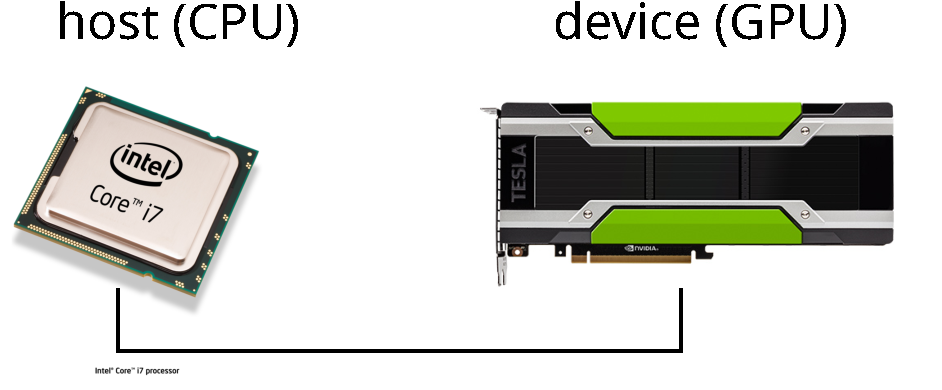
\includegraphics[width=0.6\textwidth]{out/pdf/svg/cpu_gpu_1.pdf}
  \end{center}
  
\end{frame}

%=================================
\section{Kernels}
%=================================

%%%%%%%%%%%%%%%%% 
\begin{frame}[fragile]
  \frametitle{Two things you need to learn first:
    writing and launching kernels}
  \begin{itemize}
  \item a ``GPU kernel'' (or simply a ``kernel'') is a function that runs on GPU
\begin{lstlisting}
@{\ao{\tt \_\_global\_\_}}@ void f(...) { ... }
\end{lstlisting}
\item syntactically, 
  a kernel is an ordinary C++ function that returns nothing ({\tt void}),
  except for the {\ao{\tt \_\_global\_\_}} keyword

\item a host launches a kernel specifying the number of threads.
\begin{lstlisting}
f@\ao{<<<{\it nb},{\it bs}>>>}@(...);
\end{lstlisting}
will create ({\it nb} $\times$ {\it bs}) CUDA threads,
each executing f(...)
\end{itemize}

\begin{center}
  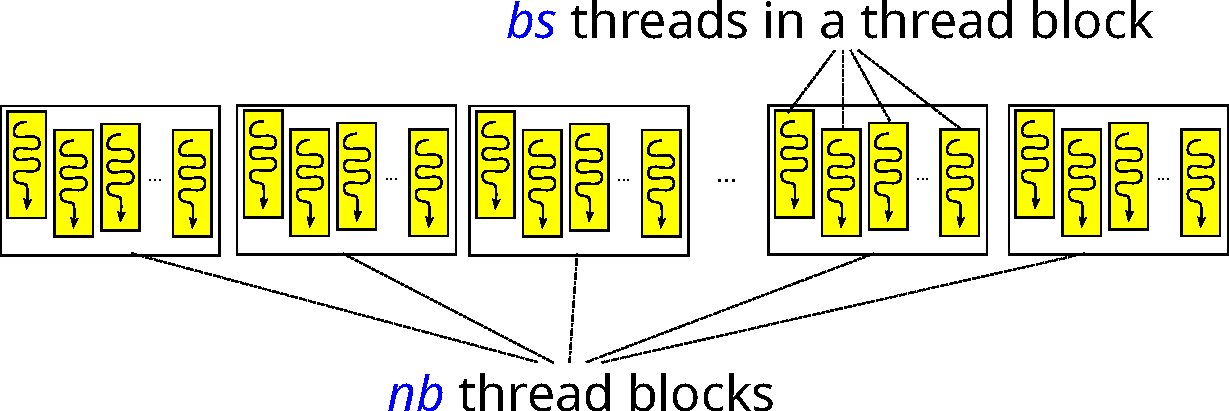
\includegraphics[width=0.6\textwidth]{out/pdf/svg/thread_blocks_1.pdf}
\end{center}

\end{frame}

%%%%%%%%%%%%%%%%% 
\begin{frame}[fragile]
  \frametitle{Launching a kernel $\approx$ parallel loop}
\begin{itemize}
  \item launching a kernel, like
\begin{lstlisting}
f@\ao{<<<{\it nb},{\it bs}>>>}@(...);
\end{lstlisting}

\item $\approx$ executing the following loop in parallel
  (on GPU, of course)
\begin{lstlisting}
for (i = 0; i < @{\it nb}@ * @{\it bs}@; i++) {
  f(...); // CUDA thread
}
\end{lstlisting}

\item []

  \begin{center}
    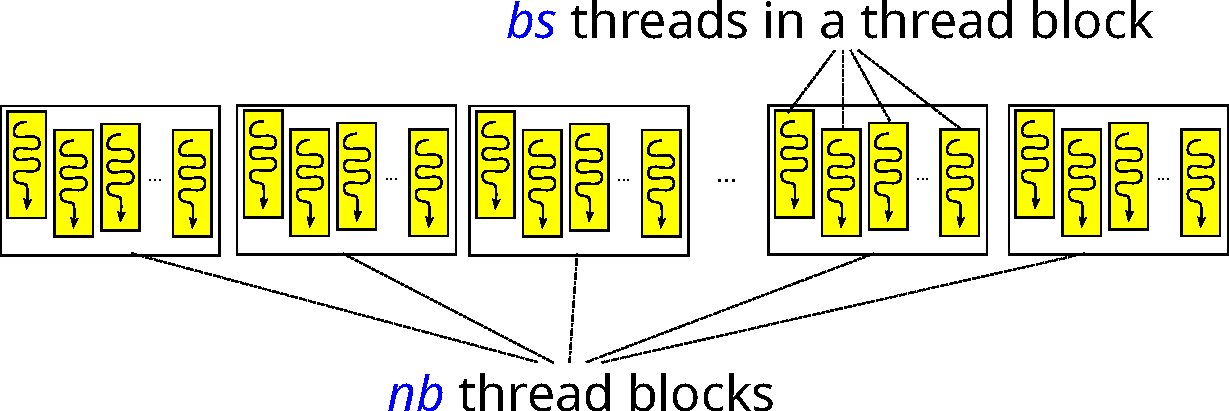
\includegraphics[width=0.8\textwidth]{out/pdf/svg/thread_blocks_1.pdf}
  \end{center}
\end{itemize}
\end{frame}

%%%%%%%%%%%%%%%%% 
\begin{frame}[fragile]
\frametitle{A simplest example}
\begin{itemize}
\item [] writing a kernel
\begin{lstlisting}
__global__ void cuda_thread_fun(int n) {
  int i        = @\ao{\tt blockDim.x * blockIdx.x + threadIdx.x}@;
  int nthreads = @\ao{\tt gridDim.x * blockDim.x}@;
  if (i < n) {
    printf("hello I am CUDA thread %d out of %d\n", i, n);
  }
}
\end{lstlisting}

\item [] and launching it
\begin{lstlisting}
int thread_block_sz = 64;
int n_thread_blocks = (n + thread_block_sz - 1) / thread_block_sz;
cuda_thread_fun<<<n_thread_blocks,thread_block_sz>>>(n);
\end{lstlisting}

\item [] will print hello $n$ times
\begin{lstlisting}
hello I am CUDA thread 0 out of @$n$@
   ...
hello I am CUDA thread @$n-1$@ out of @$n$@
\end{lstlisting}
{\it note: the order is unpredictable}
\end{itemize}
\end{frame}

%%%%%%%%%%%%%%%%% 
\begin{frame}[fragile]
  \frametitle{A CUDA thread is not like an OpenMP thread}
  \begin{itemize}
  \item launching 10000 CUDA threads is quite common and efficient
\begin{lstlisting}
f<<<1024,256>>(...);      
\end{lstlisting}

\item launching 10000 threads on CPU is almost always a bad idea
\item below is ``semantically'' similar to the above  
\begin{lstlisting}
#pragma omp parallel
  f();
\end{lstlisting}
\begin{lstlisting}
@\aka{\tt OMP\_NUM\_THREADS=262144}@ ./a.out
\end{lstlisting}
but what happens inside is very different

\item CPU way of doing this was:
\begin{lstlisting}
#pragma omp parallel @\ao{\tt for}@
for (i = 0; i < 1024 * 256; i++) { f(); }
\end{lstlisting}
\begin{lstlisting}
@\ao{{\tt OMP\_NUM\_THREADS=}{\it a modest number}}@ ./a.out
\end{lstlisting}
{\it a modest number} $=$ typically the actual number of cores
\end{itemize}

\end{frame}

%%%%%%%%%%%%%%%%% 
\begin{frame}[fragile]
  \frametitle{A kernel call and the host overlap but two kernel calls do not}
  \begin{itemize}
  \item when you call a kernel,
    the host continues execution without waiting for it to finish
  \item two kernel calls are serialized on the GPU side, by default
  \item {\tt cudaDeviceSynchronize()} is an API to wait for the kernel to finish
  \end{itemize}

  \begin{columns}
    \begin{column}{0.35\textwidth}
\begin{lstlisting}
h0();
g0<<<...,...>>>();
h1();
g1<<<...,...>>>(); 
h2();
g2<<<...,...>>>(); 
cudaDeviceSynchronize();
h3();
\end{lstlisting}
    \end{column}
    \begin{column}{0.65\textwidth}
\begin{itemize}
\item {\tt g0} may overlap with {\tt h1} and {\tt h2}
\item {\tt g0} and {\tt g1} do not overlap because of GPU serializes them by default
\item {\tt h3} does not overlap with anything because of
  {\tt cudaDeviceSynchronize()}
\end{itemize}
\end{column}    
\end{columns}
  
\end{frame}

  
%%%%%%%%%%%%%%%%% 
\begin{frame}[fragile]
\frametitle{About thread IDs}
\begin{itemize}
\item for each thread to determine what to do, it
  needs a unique ID (the loop index)
\item you get it from \ao{\tt gridDim, block\{Dim,Idx\}} and \ao{\tt threadIdx}
\item when you launch a kernel by
\begin{lstlisting}
f<<<nb,bs>>>(...);
\end{lstlisting}

\begin{center}
  
\includegraphics[width=0.6\textwidth]{out/pdf/svg/thread_blocks_2.pdf}
\end{center}

\begin{itemize}
\item {\tt block\ao{Dim}.x} = {\it bs} (the thread block size)
\item {\tt grid\ao{Dim}.x} = {\it nb} (the number of blocks $=$ the ``grid'' size)
\end{itemize}
and
\begin{itemize}
\item {\tt thread\ao{Idx}.x} = the thread ID within the block
  ($\in [0, \mbox{\it bs})$)
\item {\tt block\ao{Idx}.x} = the thread's block ID
  ($\in [0, \mbox{\it nb})$)
\end{itemize}
\end{itemize}
\end{frame}


%%%%%%%%%%%%%%%%% 
\begin{frame}[fragile]
\frametitle{{\it nb} and {\it bs} can be 2/3-Dimensional}
\begin{itemize}
\item as suggested by {\tt .x}, a block and the grid
  can be multidimensional (up to 3D, of {\tt .x, .y, .z})
  and the previous code assumes they are 1D
  
\item extension to multidimensional block/grid is
  straightforward

\item 1D:
\begin{lstlisting}
int nb = 100;
int bs = 256
f<<<nb,bs>>>(...); // 100*256 threads
\end{lstlisting}

\item 2D:
\begin{lstlisting}
dim3 nb(10,10);
dim3 bs(8,32);
f<<<nb,bs>>>(...); // 10*10*8*32 threads
\end{lstlisting}

\item 3D:
\begin{lstlisting}
dim3 nb(10,5,2);
dim3 bs(8,8,4);
f<<<nb,bs>>>(...); // 10*5*2*8*8*4 threads
\end{lstlisting}
\end{itemize}
\end{frame}


%%%%%%%%%%%%%%%%% 
\begin{frame}[fragile]
\frametitle{SpMV in CUDA}
\begin{itemize}
  \item original serial code
\begin{lstlisting}
for (k = 0; k < A.nnz; k++) {
  i,j,Aij = A.elems[k];
  y[i] += Aij * x[j];
}
\end{lstlisting}

\item write a kernel that
  \ao{\it works on a single non-zero element}
\begin{lstlisting}
__global__ spmv_dev(A, x, y) {
  k = @\ao{\tt blockDim.x * blockIdx.x + threadIdx.x}@; // thread id
  if (k < A.nnz) {
    i,j,Aij = A.elems[k];
    y[i] += Aij * x[j];   }   }
\end{lstlisting}

\item and launch it with $\geq$ {\tt nnz} threads
  \aka{\it (we're not done yet)}
\begin{lstlisting}
@\aka{\tt spmv*}@(A, x, y) {
  int bs = 256;
  int nb = (A.nnz + bs - 1) / bs;    
  spmv_dev<<<nb,bs>>(A, x, y);  }
\end{lstlisting}

\item similarly simple for CSR version

\end{itemize}
\end{frame}

%%%%%%%%%%%%%%%%% 
\begin{frame}[fragile]
\frametitle{We're not done yet}
\begin{itemize}
\item this code
\begin{lstlisting}
__global__ spmv_dev(A, x, y) {
  k = blockDim.x * blockIdx.x + threadIdx.x;
  if (k < nnz) {
    i,j,Aij = @\mura{A.elems[k]}@;
    @\aka{\tt y[i] +=}@ Aij * @\mura{x[j]}@;
  }
}
\end{lstlisting}
does not work yet

\begin{enumerate}
\item the device \mura{cannot access elements}
  of {\tt A, x} and {\tt y} on the host
\item there is a race condition when updating \aka{\tt y[i]}
\end{enumerate}
\end{itemize}
\end{frame}

%%%%%%%%%%%%%%%%% 
\begin{frame}[fragile]
  \frametitle{Keywords for functions}
\begin{itemize}
\item {\tt \_\_global\_\_}, {\tt \_\_device\_\_}, {\tt \_\_host\_\_}
  % $T$ $f$(args) { ... }
\item []
  \begin{tabular}{|l|l|l|}\hline
     & callable from & code runs on \\\hline
    {\tt \_\_global\_\_} & host/device & device \\
    {\tt \_\_device\_\_} & device      & device \\
    {\tt \_\_host\_\_}   & host        & host   \\\hline
  \end{tabular}

\item {\tt \_\_global\_\_} functions cannot return a value
  (must be {\tt void})

\item you can have both {\tt \_\_host\_\_} and {\tt \_\_device\_\_}
  in front of a definition, which
  generates two versions (device and host)
\end{itemize}
\end{frame}

%%%%%%%%%%%%%%%%% 
\begin{frame}[fragile]
  \frametitle{Macros}
  \begin{itemize}
  \item convenient when writing a single file that works both on CPU and GPU
    
\item {\tt \_\_NVCC\_\_} : a macro defined when compiled by nvcc
\begin{lstlisting}
#ifdef __NVCC__
  // GPU implementation
#else
  // CPU implementation
#endif    
\end{lstlisting}
  
\item {\tt \_\_CUDA\_ARCH\_\_} : a macro defined when copiled for device
\begin{lstlisting}
__device__ __host__ f(...) {
#ifdef __CUDA_ARCH__
  // device code
#else
  // host code
#endif
}
\end{lstlisting}
\end{itemize}
\end{frame}

%=================================
\section{Threads and thread blocks}
%=================================

%%%%%%%%%%%%%%%%%
\begin{frame}
\frametitle{Threads and thread blocks (recap)}
\begin{itemize}
\item a kernel specifies the action of {\it a} CUDA thread
\item when you launch a kernel you specify
  \begin{itemize}
  \item the number of thread blocks (\ao{\it nb}) and
  \item the thread block size $=$ the number of threads in a single thread block (\ao{\it bs}),
  \end{itemize}
  to effectively create (\ao{{\it nb} $\times$ {\it bs}}) threads
\end{itemize}

\begin{center}
  
\includegraphics[width=0.6\textwidth]{out/pdf/svg/thread_blocks_2.pdf}
\end{center}

\ao{\it but why you need two separate numbers?}

\end{frame}

%%%%%%%%%%%%%%%%% 
\begin{frame}
  \frametitle{Why two numbers ({\it bs} and {\it nb})?}

  \ao{\it a single thread block is sent to a single SM
    and stays there until it finishes}

  \begin{center}
    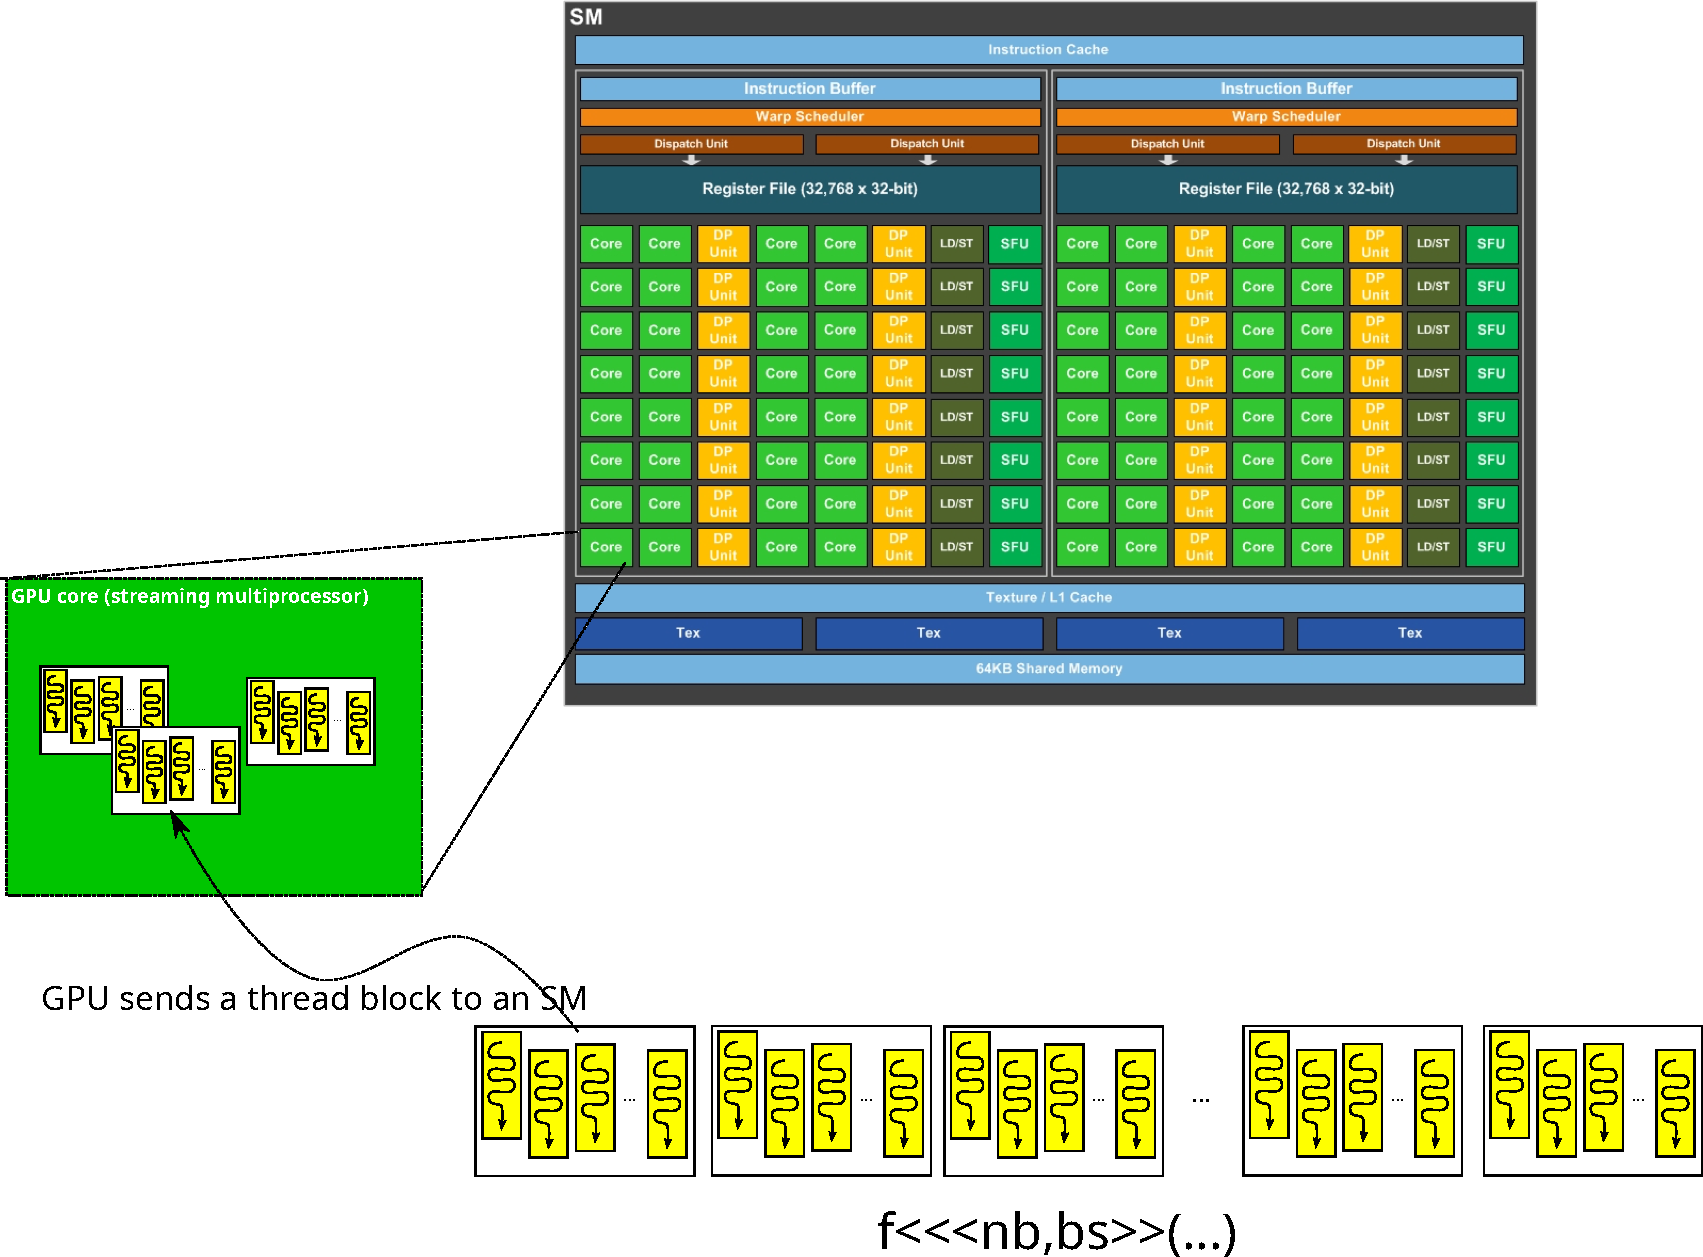
\includegraphics[width=0.6\textwidth]{out/pdf/svg/sm_and_blocks_1.pdf}
  \end{center}
\end{frame}

%%%%%%%%%%%%%%%%% 
\begin{frame}
  \frametitle{The way thread block boundaries are {\it semantically} visible}
  \begin{itemize}
  \item<2-> CUDA API exposes \ao{\it ``shared memory''}, a small cache-like
    memory only shared within a single thread block
  \item<3-> CUDA API exposes some synchronization/coordination primitives
    (e.g., {\tt \_\_syncthreads()} or reduction) only usable within
    a single thread block
  \item<4-> unless you rely on these primitives,
    choosing the thread block size is largely a performance
    (not a correctness) issue
  \end{itemize}
  \begin{center}
    \only<1>{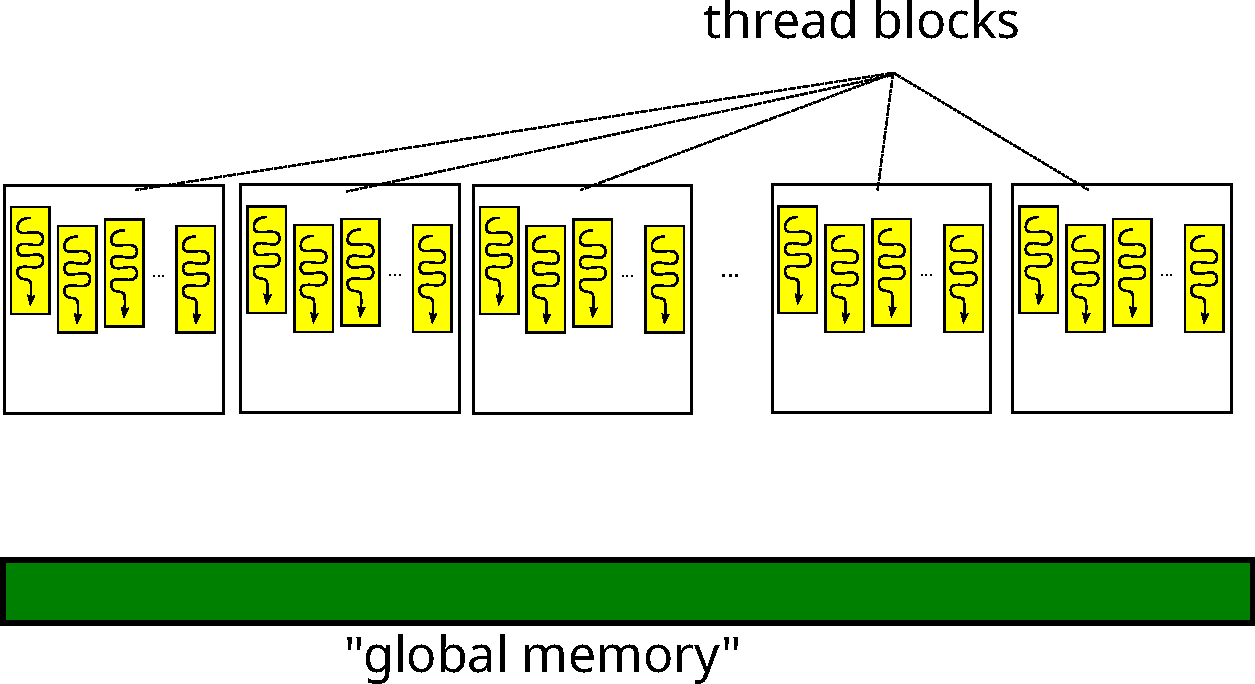
\includegraphics[width=0.6\textwidth]{out/pdf/svg/cuda_shmem_1.pdf}}%
    \only<2>{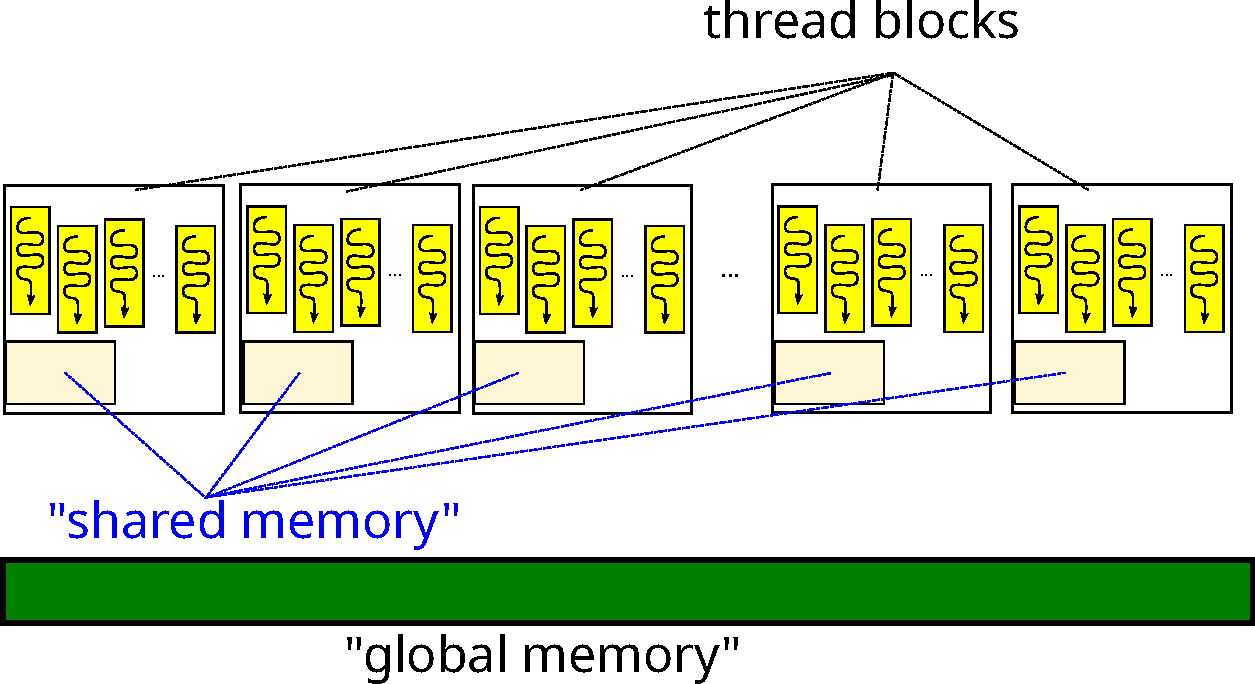
\includegraphics[width=0.6\textwidth]{out/pdf/svg/cuda_shmem_2.pdf}}%
    \only<3->{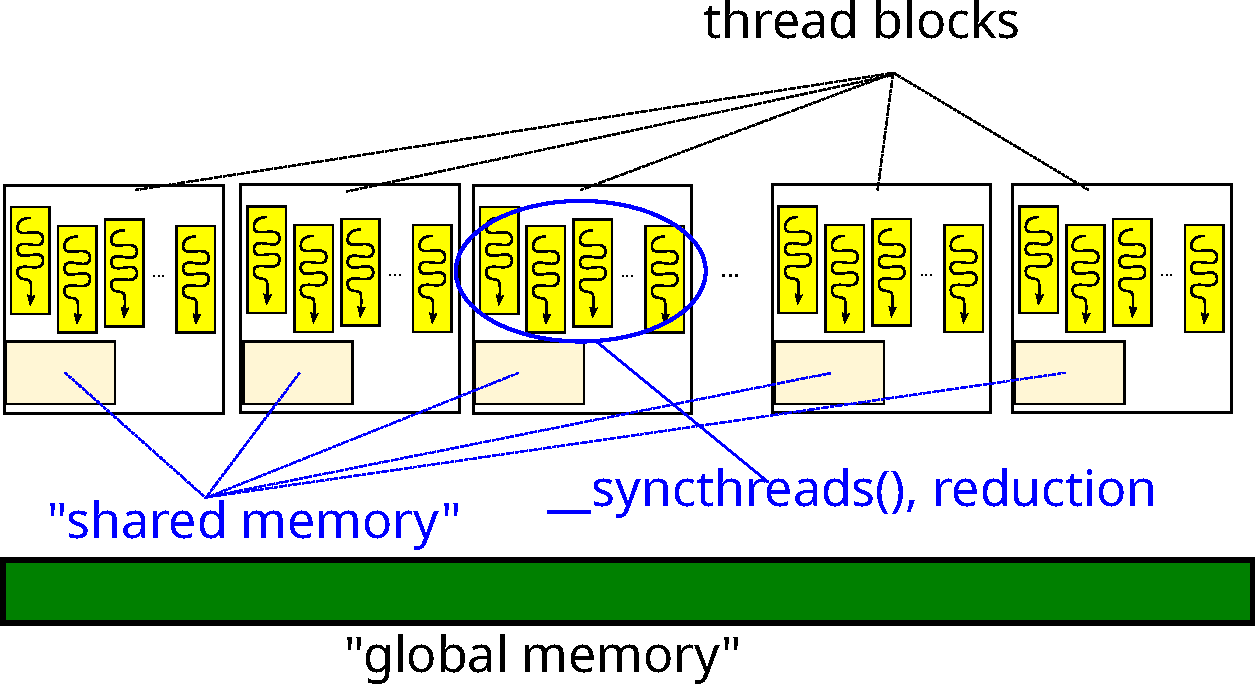
\includegraphics[width=0.6\textwidth]{out/pdf/svg/cuda_shmem_3.pdf}}%
  \end{center}
\end{frame}

% =================================
\section{Communicating data between host and device}
%=================================

%%%%%%%%%%%%%%%%% 
\begin{frame}[fragile]
\frametitle{Moving data between host and device}
\begin{itemize}
\item host and device memory are \aka{\it separate}
\item the device cannot access data on the host and vice versa
  (at least not directly by hardware until recently)
\item i.e., the following does not work
\begin{lstlisting}
double a[n];
f<<<nb,bs>>>(a);
\end{lstlisting}

\begin{lstlisting}
__global__ f(double * a) {
  ... a[i] ... // this will segfault
}
\end{lstlisting}
\end{itemize}

\begin{center}
\only<1>{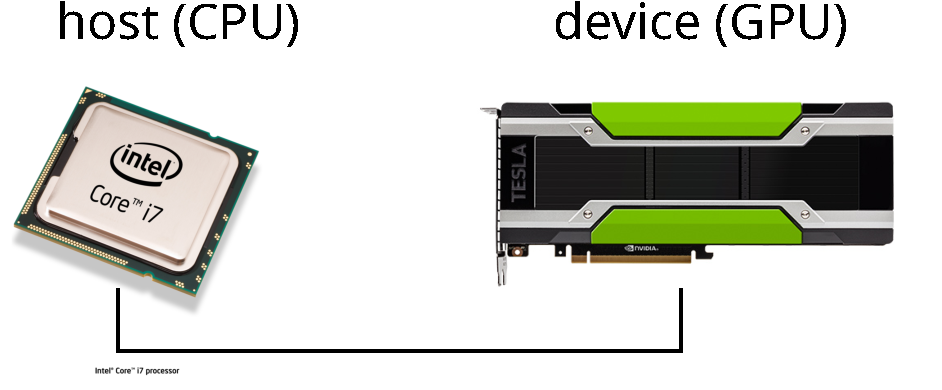
\includegraphics[width=0.6\textwidth]{out/pdf/svg/cpu_gpu_1.pdf}}%
\only<2->{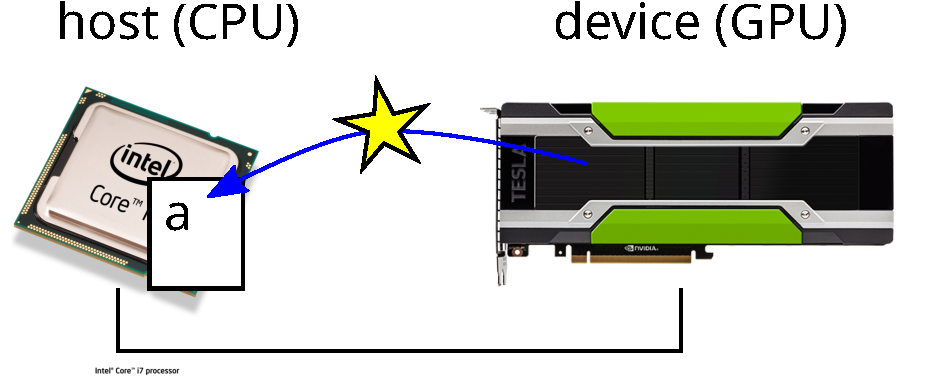
\includegraphics[width=0.6\textwidth]{out/pdf/svg/cpu_gpu_3.pdf}}
\end{center}
\end{frame}

%%%%%%%%%%%%%%%%% 
\begin{frame}[fragile]
  \frametitle{Two more things you must master:
    {\tt cudaMalloc} and {\tt cudaMemcpy}}
\begin{itemize}
\item you need to
  \begin{enumerate}
  \item<2-> allocate data on device (by \ao{\tt cudaMalloc})
    $\rightarrow$ {\it device memory}
  \item<3-> move data between the host and the device (by \ao{\tt cudaMemcpy})
  \item<4-> give the kernel the pointer to the device memory
  \end{enumerate}
\item<5-> note: call \ao{\tt cudaMalloc} and \ao{\tt cudaMemcpy}
  on the host, not on the device
\end{itemize}

  \begin{center}
\only<1>{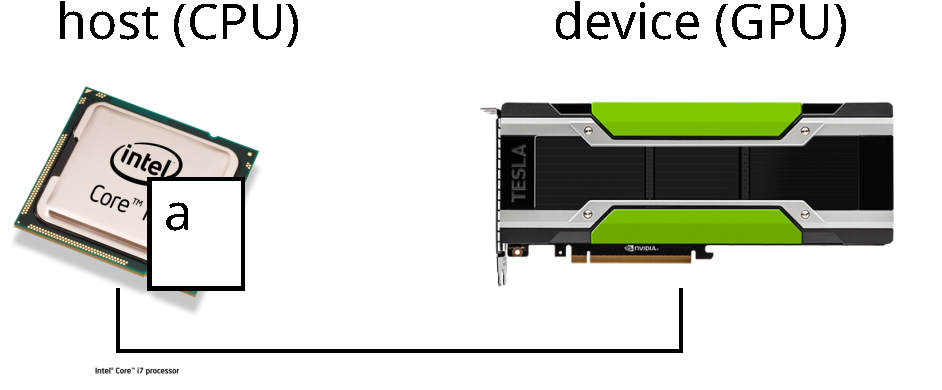
\includegraphics[width=0.6\textwidth]{out/pdf/svg/cpu_gpu_2.pdf}}%
\only<2>{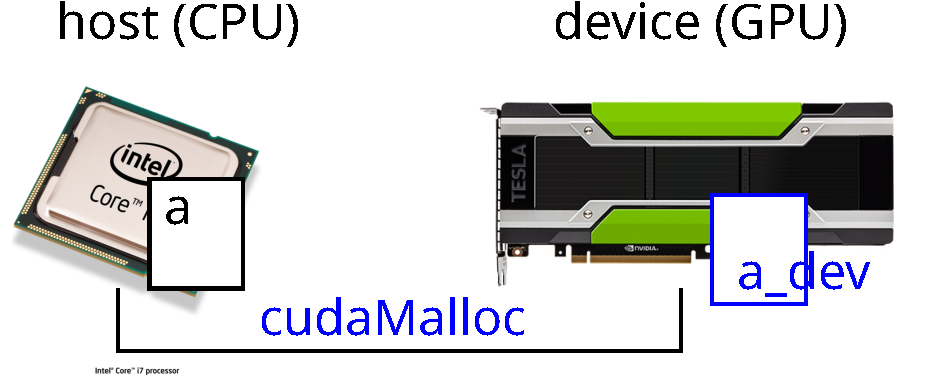
\includegraphics[width=0.6\textwidth]{out/pdf/svg/cpu_gpu_4.pdf}}%
\only<3->{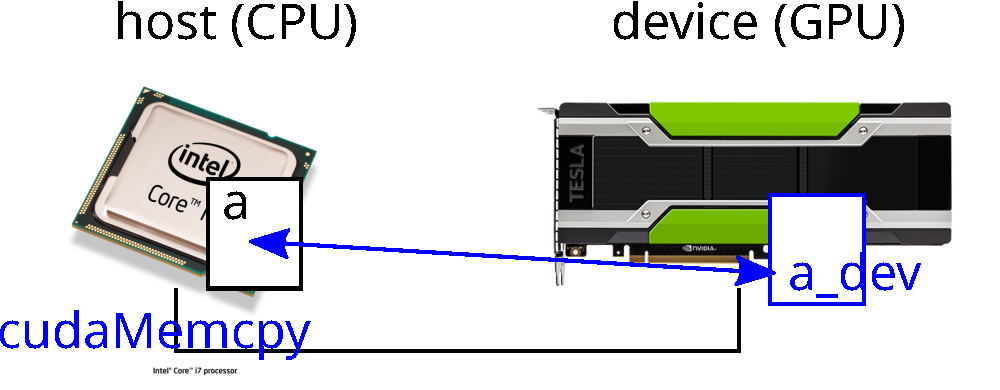
\includegraphics[width=0.6\textwidth]{out/pdf/svg/cpu_gpu_5.pdf}}
  \end{center}
\end{frame}

%%%%%%%%%%%%%%%%% 
\begin{frame}[fragile]
\frametitle{Typical steps to send data to the device}
\begin{enumerate}
\item allocate data of the same size both on host and device
\begin{lstlisting}
double * a = ...;  // any valid address will do (malloc, &variable, etc.)
double * a_dev = 0;
@\ao{\tt cudaMalloc}@((void **)&a_dev, sz);
\end{lstlisting}

\item the host works on the host data
\begin{lstlisting}
for ( ... ) { a[i] = ... } // whatever initialization you need
\end{lstlisting}

\item copy the data to the device
\begin{lstlisting}
@\ao{\tt cudaMemcpy}@(a_dev, a, sz, @\ao{\tt cudaMemcpyHostToDevice}@);
\end{lstlisting}

\item pass the device pointer to the kernel 
\begin{lstlisting}
f<<<nb,bs>>>(@\ao{\tt a\_dev}@, ...)
\end{lstlisting}

\item often a good idea to have
  a struct encapsulating both pointers
  {\small
\begin{lstlisting}
typedef struct {
  double * a;     // host pointer
  double * a_dev; // device pointer
   ...          } my_struct;
\end{lstlisting}}
\end{enumerate}
\end{frame}

%%%%%%%%%%%%%%%%% 
\begin{frame}[fragile]
\frametitle{Typical steps to retrieve the result}
\begin{enumerate}
\item allocate data of the same size both on host and device
\begin{lstlisting}
double * r = ... ;
double * r_dev = 0;
@\ao{\tt cudaMalloc}@((void **)&r_dev, sz);
\end{lstlisting}

\item pass the device pointer to the kernel 
\begin{lstlisting}
f<<<nb,bs>>>(..., r_dev);
\end{lstlisting}

\item copy the data to the host
\begin{lstlisting}
cudaMemcpy(r, r_dev, sz, cudaMemcpyDeviceToHost);
\end{lstlisting}
\end{enumerate}
\end{frame}

%%%%%%%%%%%%%%%%% 
\begin{frame}
  \frametitle{Unified Memory}
  \begin{itemize}
  \item recent NVIDIA GPUs support \ao{Unified Memory} that eliminate the need for
    explicit data movement between host and device memory
    and dual pointer management
  \item at the heart of it is \ao{\tt cudaMallocManaged}, which is like
    {\tt cudaMalloc} but is directly accessible from host CPU too
  \end{itemize}
\end{frame}


%%%%%%%%%%%%%%%%% 
\begin{frame}[fragile]
\frametitle{Typical steps to send data to the device with Unified Memory}
\begin{enumerate}
\item allocate data of the same size both on host and device
\begin{lstlisting}
double * a = 0;
@\ao{\tt cudaMallocManaged}@((void **)&a, sz);
\end{lstlisting}

\item the host works on the host data
\begin{lstlisting}
for ( ... ) { a[i] = ... } // whatever initialization you need
\end{lstlisting}

\item pass the pointer to the kernel 
\begin{lstlisting}
f<<<nb,bs>>>(@\ao{\tt a}@, ...)
\end{lstlisting}

\end{enumerate}
\end{frame}


%%%%%%%%%%%%%%%%% 
\begin{frame}[fragile]
\frametitle{Typical steps to retrieve the result with Unified Memory}
\begin{enumerate}
\item allocate data with {\tt cudaMallocManaged}
\begin{lstlisting}
double * r = 0;
@\ao{\tt cudaMallocManaged}@((void **)&r, sz);
\end{lstlisting}

\item pass the device pointer to the kernel 
\begin{lstlisting}
f<<<nb,bs>>>(..., r);
\end{lstlisting}

\item make sure threads finished their work
\begin{lstlisting}
cudaDeviceSynchronize();
\end{lstlisting}
\end{enumerate}
\end{frame}

% =================================
\section{Data sharing among threads in the device}
%=================================

%%%%%%%%%%%%%%%%% 
\begin{frame}
\frametitle{Data sharing among threads in the device}
\begin{itemize}
\item basics :
  memory allocated via {\tt cudaMalloc(Managed)?}
  {\it are shared among all threads}
  \ao{\it (global memory)}
  \begin{itemize}
  \item a write by a thread will be visible to all others (sooner or later)
  \end{itemize}

\item \ao{\it shared memory} : 
  \begin{itemize}
  \item hardware terms: a small on-chip memory as fast as caches,
    not coherent across SMs
  \item software view:
    memory shared only within a thread block
  \end{itemize}

\item other weirder memory types not covered in the lecture
  (constant and texture)
\end{itemize}

\begin{center}
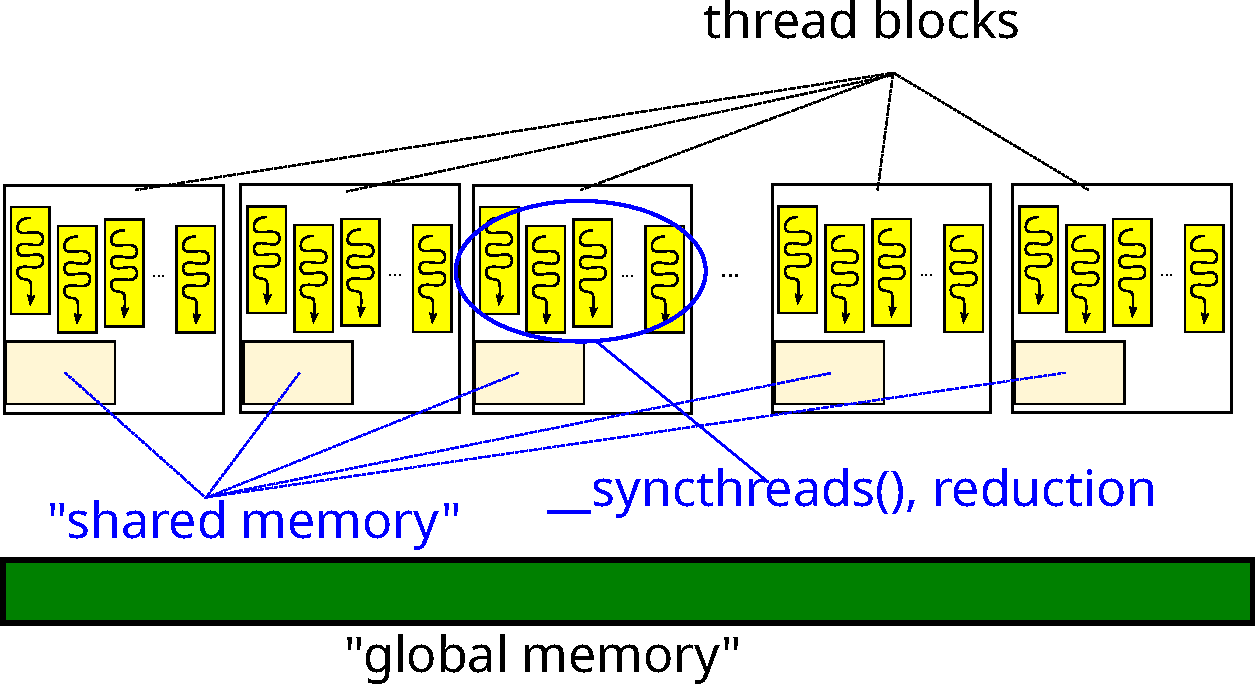
\includegraphics[width=0.5\textwidth]{out/pdf/svg/cuda_shmem_3.pdf}
\end{center}

\end{frame}

%%%%%%%%%%%%%%%%% 
\begin{frame}[fragile]
\frametitle{How to resolve race conditions on global/shared memory?}
\begin{itemize}
\item CUDA threads run concurrently
  so they are susceptible to race conditions as in CPUs
\begin{lstlisting}
__global__ spmv_dev(A, x, y) {
  k = @\ao{\tt blockDim.x * blockIdx.x + threadIdx.x}@; // thread id
  if (k < nnz) {
    i,j,Aij = A.elems_dev[k];
    @\aka{\tt y[i] +=}@ Aij * x[j];
  }
}
\end{lstlisting}
\end{itemize}
\end{frame}

%%%%%%%%%%%%%%%%% 
\begin{frame}
\frametitle{Resolving race condition on CUDA}
\begin{itemize}
\item \ao{atomic accumulations} ({\tt atomicAdd} and other functions)
\item forget about mutual exclusion (no {\tt \#pragma omp critical} equivalent)
\item \ao{barrier synchronization},
  upon which you can built reductions
\item \ao{reduction}, \mura{\it but only within a single thread block}
\end{itemize}

\begin{center}
  {\footnotesize
  \begin{tabular}{|l|l|l|}\hline
                    & OpenMP  & CUDA \\\hline
atomic accumulation & pragma {\tt atomic} & atomicAdd \\
mutual exclusion & pragma {\tt critical} &  \\
                 & or {\tt omp\_lock\_t} &  \\
barrier & pragma {\tt barrier} & cooperative thread group \\
reduction & pragma {\tt reduction} & only within a thread block, \\
                    &  & or DIY with barrier \\\hline    
\end{tabular}}
\end{center}

\end{frame}

%%%%%%%%%%%%%%%%% 
\begin{frame}[fragile]
  \frametitle{Atomic accumulations}
  \begin{itemize}
  \item consider the following (trivial) example
\begin{lstlisting}
int * a;      
cudaMallocManaged(&a, sizeof(int) * nb * bs);
for (i=0; i<nb*bs; i++) a[i] = 1;
sum<<<nb,bs>>>(a);
cudaDeviceSynchronize();
printf("sum = %d\n", a[0]);
\end{lstlisting}%$
\item the goal is to guarantee it always prints the sum of all elements
  in the array ($=$ {\tt nb} $\times$ {\tt bs})
\item a race-prone version
\begin{lstlisting}
__global__ void f(int * a) {
  int i = @{\it thread id}@;
  if (i > 0) a[0] += a[i];
}
\end{lstlisting}  
\end{itemize}
\end{frame}

%%%%%%%%%%%%%%%%% 
\begin{frame}[fragile]
\frametitle{Atomic accumulations}
\begin{itemize}
\item atomic accumulations are supported by the hardware and CUDA API
  \begin{itemize}
  \item {\tt atomicAdd({\it p}, {\it x})}
    $\approx$
\begin{lstlisting}
#pragma omp atomic
  @{\tt *{\it p} += {\it x}}@
\end{lstlisting}
in OpenMP
  \item search the CUDA toolkit documentation for ``atomicAdd''
  \end{itemize}
\item there are other primitives, such as compare-and-swap
\item fix our example
\begin{lstlisting}
__global__ void f(int * a) {
  int i = @{\it thread id}@;
  if (i > 0) atomicAdd(&a[0], a[i]);
}
\end{lstlisting}
\end{itemize}
\end{frame}

%%%%%%%%%%%%%%%%% 
\begin{frame}[fragile]
\frametitle{A working version of COO SpMV}
\begin{itemize}
\item []
\begin{lstlisting}
__global__ spmv_dev(A, x, y) {
  k = @\ao{\it thread id}@;
  if (k < nnz) {
    i,j,Aij = A.elems_dev[k];
    atomicAdd(@\ao{\tt \&y[i]}@, Aij * x[j]);
  }
}
\end{lstlisting}

\item make sure {\tt A.elems\_dev}, {\tt x} and {\tt y}
  point to device memory (not shown) 

\item note: CSR is simpler to work with
  if you don't parallelize within a row
\end{itemize}
\end{frame}

%%%%%%%%%%%%%%%%% 
\begin{frame}
\frametitle{Barrier synchronization}
\begin{itemize}
\item barrier is a mechanism to ensure
  ``all threads reached a point''
\item useful to ensure changes made by a thread is visible all others
\item CUDA used to support barriers only within a single thread block
  ({\tt \_\_syncthreads()})
\item it now supports barriers for all threads 
  \href{https://docs.nvidia.com/cuda/cuda-c-programming-guide/index.html\#cooperative-groups}{(C. Cooperative Groups)}
\end{itemize}

\begin{center}
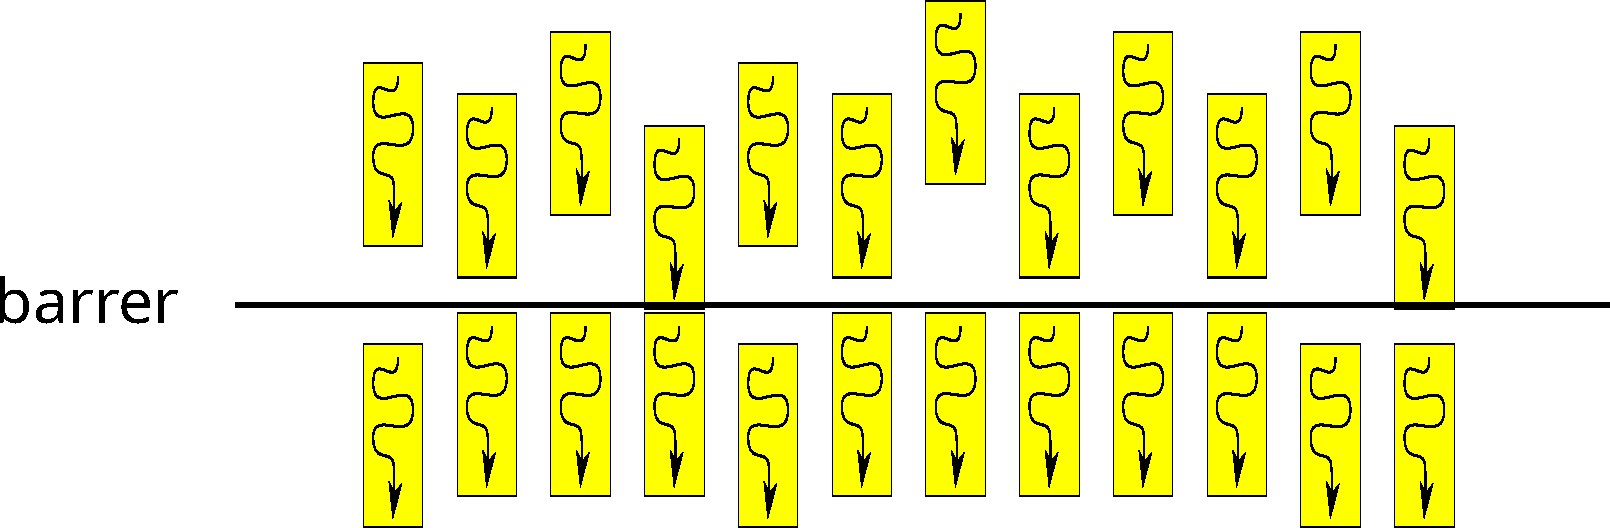
\includegraphics[width=0.7\textwidth]{out/pdf/svg/barrier.pdf}
\end{center}
\end{frame}

%%%%%%%%%%%%%%%%% 
\begin{frame}[fragile]
\frametitle{Cooperative groups (1)}
\begin{itemize}
\item (important) when using the following features, launch a kernel by
\begin{lstlisting}
void * args[] = { a0, a1, ... };
cudaLaunchCooperativeKernel((void *)f, nb, bs, args);
\end{lstlisting}
instead of the ordinary
\begin{lstlisting}
f<<<nb,bs>>>(a0, a1, ...);
\end{lstlisting}

\item common setup
\begin{lstlisting}
#include <cooperative_groups.h>
namespace cg = cooperative_groups; // save typing
\end{lstlisting}
\end{itemize}
\end{frame}

%%%%%%%%%%%%%%%%% 
\begin{frame}[fragile]
\frametitle{Cooperative groups (2)}
\begin{itemize}
\item data representing a group
\begin{lstlisting}
cg::grid_group g = cg::this_grid(); // all threads
\end{lstlisting}
\begin{lstlisting}
cg::thread_block g = cg::this_thread_block(); // thread block
\end{lstlisting}

\item barrier synchronization
\begin{lstlisting}
g.sync(); // barrier all theads in g participate
\end{lstlisting}

\item group actually provides a cleaner way to know thread ID and number of threads
\begin{lstlisting}
unsigned long long idx = g.thread_rank(); // my ID in g
unsigned long long nth = g.size(); // num threads in g
\end{lstlisting}
\end{itemize}
\end{frame}

%%%%%%%%%%%%%%%%% 
\begin{frame}[fragile]
  \frametitle{Building reduction on barrier}
\begin{center}
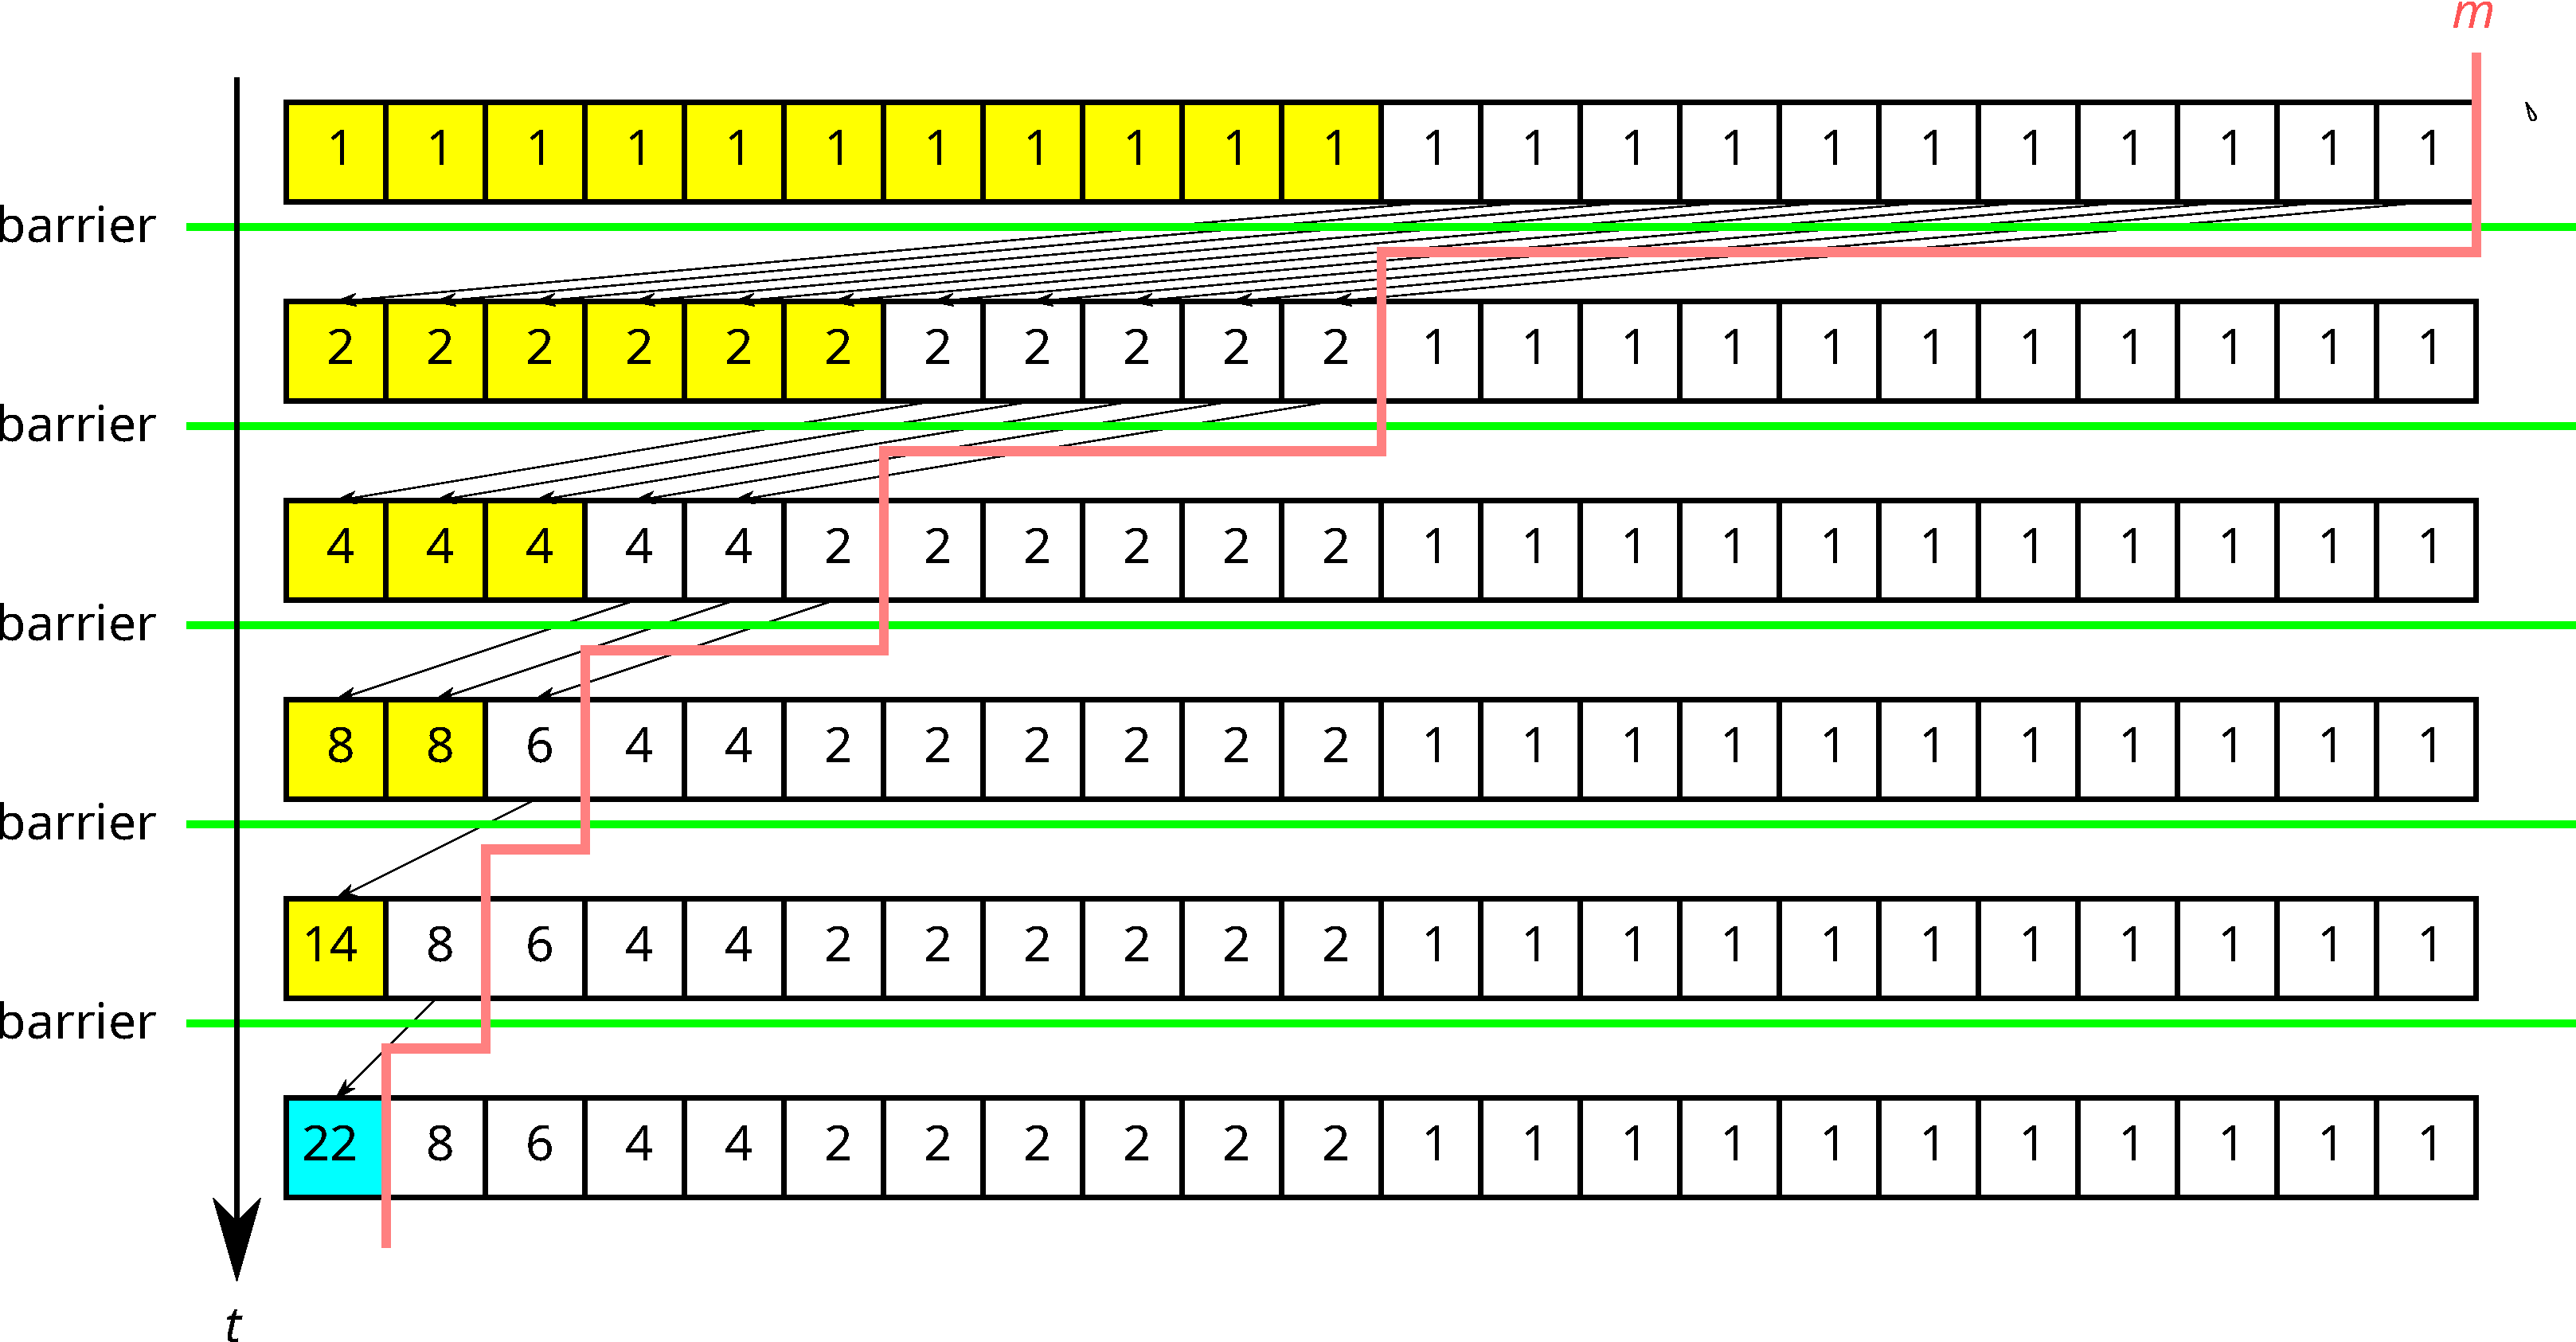
\includegraphics[width=0.55\textwidth]{out/pdf/svg/reduction_barrier.pdf}
\end{center}
  \begin{columns}
    \begin{column}{0.55\textwidth}
      \begin{center}
        \begin{itemize}
        \item []
\begin{lstlisting}
__global__
void sum(double * c, long n) {
  // return c[0] + .. + c[n-1]
  cg::grid_group g = cg::this_grid();
  ull i = g.thread_rank();
  ull h; // ull: unsigned long long
  for (long m = n; m > 1; m = h) {
    h = (m + 1) / 2;
    if (i + h < m) c[i] += c[i + h];
    g.sync();
  } }
\end{lstlisting}
\end{itemize}
\end{center}
\end{column}
    \begin{column}{0.47\textwidth}
\begin{itemize}
\item invariant: ``{\tt sum(c[0:$m$])} is {\it the} sum'',
  it repeats halving $m$
\item note: it may not be most efficient;
  reducing values within a single block first may be better
\end{itemize}
    \end{column}
  \end{columns}
\end{frame}

%%%%%%%%%%%%%%%%% 
\begin{frame}[fragile]
  \frametitle{CUDA shared memory}
  \begin{itemize}
  \item CUDA programs can allocate a ``shared memory'' to each thread block

\begin{lstlisting}
f<<<@{\it nb}@,@{\it bs}@,@\ao{\it S}@>>>(...);
\end{lstlisting}

\item from CUDA program's perspective, it is a memory {\it only shared within a thread block} and
  {\it only active during the thread block's lifetime}
  \begin{itemize}
  \item the term {\it shared memory} is a misnomer, IMO;
    ordinary memory you allocate via {\tt cudaMalloc}
    {\it is} shared by all threads
  \item local memory or something will be a more appropriate name
  \end{itemize}
  
\item physically, it is a cache-like memory faster than global memory

\item each SM has a fixed amount of shared memory
  (A100 : \href{https://docs.nvidia.com/cuda/ampere-tuning-guide/index.html#sm-occupancy}{164KB})
  \[ S \times \leq \mbox{shared memory per SM} \]
  % \mbox{\it bs} 
  \end{itemize}
\end{frame}

%%%%%%%%%%%%%%%%% 
\begin{frame}[fragile]
  \frametitle{Accessing CUDA shared memory}
  \begin{itemize}
  \item specify the shared memory size on a kernel call and 
    a kernel accesses it by declaring variables or arrays with
    \ao{\tt \_\_shared\_\_}
\begin{lstlisting}
__shared__ int a[n];
__shared__ char b[m];
\end{lstlisting}
\item if the data size ($n$ or $m$ above) is not a compile-time constant,
  obtain the starting address of the shared memory by
\begin{lstlisting}
extern __shared__ char whatever[];
\end{lstlisting}
\item it's your responsibility to use appropriate part of it. e.g.,
\begin{lstlisting}
int * a = (int*)whatever;
char * b = (char *)&a[n];
\end{lstlisting}
\item shared memory is a way to efficiently communicate among threads within a block
\item GPU has nowadays processor-managed caches,
  so how crucial it is to performance is somewhat changing over time
\end{itemize}
\end{frame}

\section{Choosing a block size}
%%%%%%%%%%%%%%%%% 
\begin{frame}[fragile]
  \frametitle{Choosing a good block size for performance}
  \begin{itemize}
  \item the question is, when you create a number of, say 10000, threads,
    how you divide them into thread blocks?
    \begin{lstlisting}
      f<<<1, 10000>>>(x, y, z, ...);
      f<<<10, 1000>>>(x, y, z, ...);
      f<<<100, 100>>>(x, y, z, ...);
      f<<<1000, 10>>>(x, y, z, ...);
      f<<<10000, 1>>>(x, y, z, ...);
\end{lstlisting}
    and countless other ways \ldots
  \item the goal is to run an enough number of threads {\it simultaneously}
    so they {\it utilize} the hardware capacity of an SM

\begin{center}
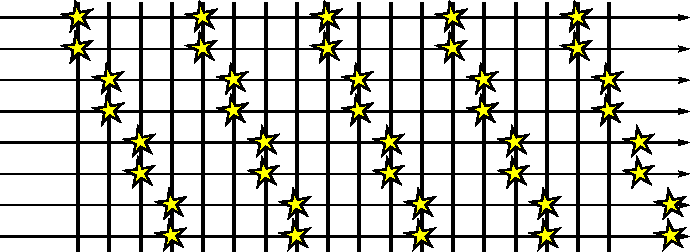
\includegraphics[width=0.5\textwidth]{out/pdf/svg/latency_4.pdf}
\end{center}
    
  \item to this end, let's understand what a GPU actually does,
    given a thread block size and the number of blocks
  \end{itemize}
\end{frame}

%%%%%%%%%%%%%%%%% 
\begin{frame}
  \frametitle{Parallelism within an SM}
  \begin{itemize}
  \item[] consists of three levels
  \item[]
    \ao{thread $\subset$ warp $\subset$ thread block $\subset$ SM}
  \end{itemize}

  \begin{itemize}
  \item<2-> a group of \ao{32} CUDA threads makes a \ao{\it warp}
  \item<3-> a group of \ao{$\left\lceil \mbox{\it bs} / 32 \right\rceil$}
    warps makes a \ao{\it thread block}
  \item<4-> and there are multiple thread blocks executing {\it simultaneously}
    on a single SM
  \end{itemize}
  \begin{center}
    \only<1>{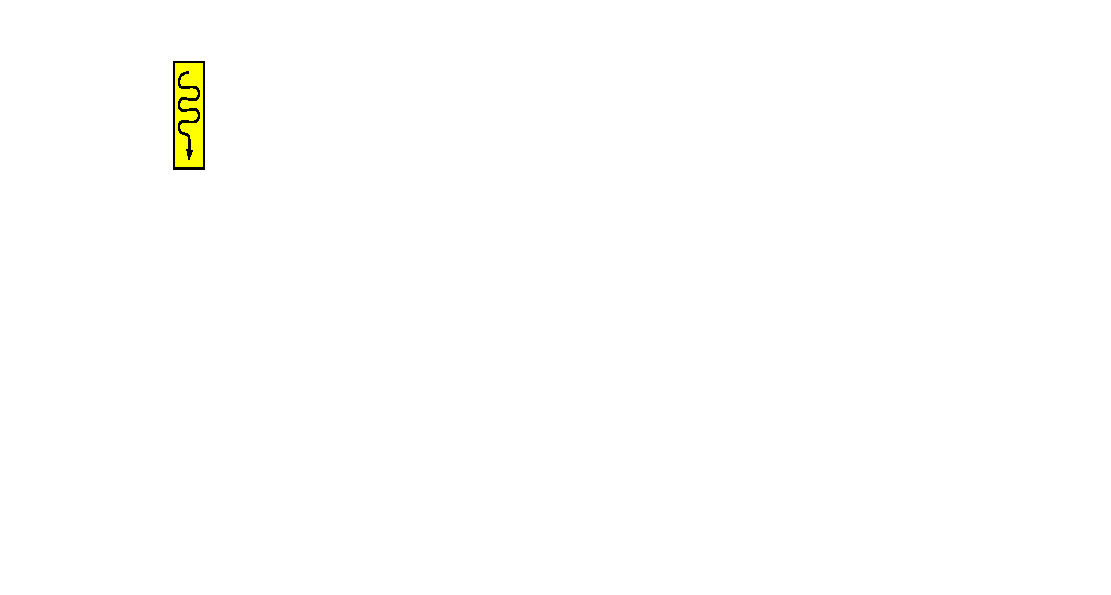
\includegraphics[width=0.7\textwidth]{out/pdf/svg/warp_block_sm_1.pdf}}%
    \only<2>{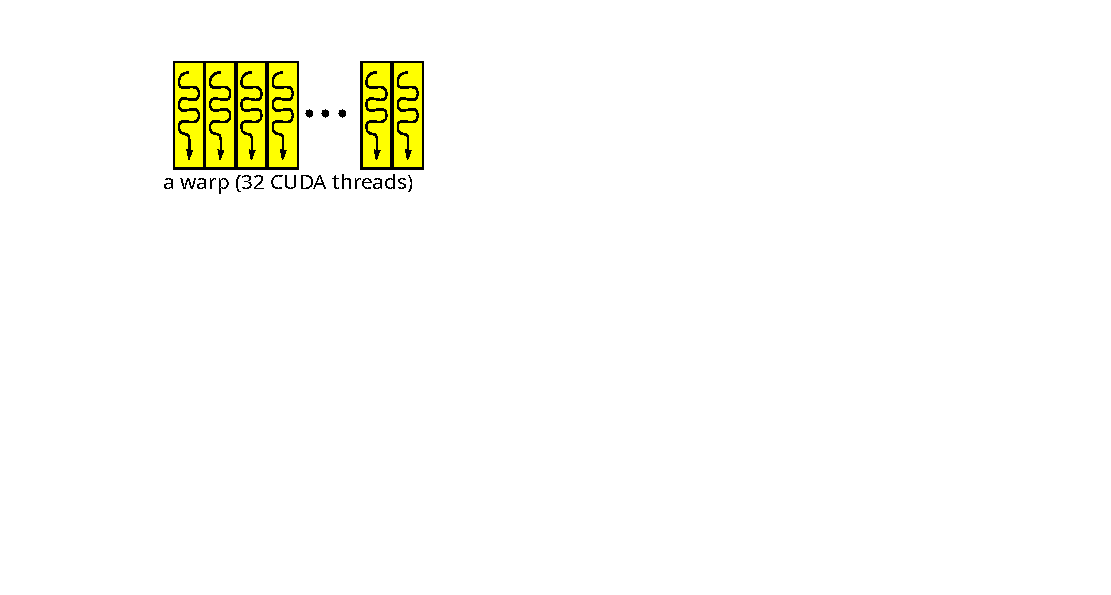
\includegraphics[width=0.7\textwidth]{out/pdf/svg/warp_block_sm_2.pdf}}%
    \only<3>{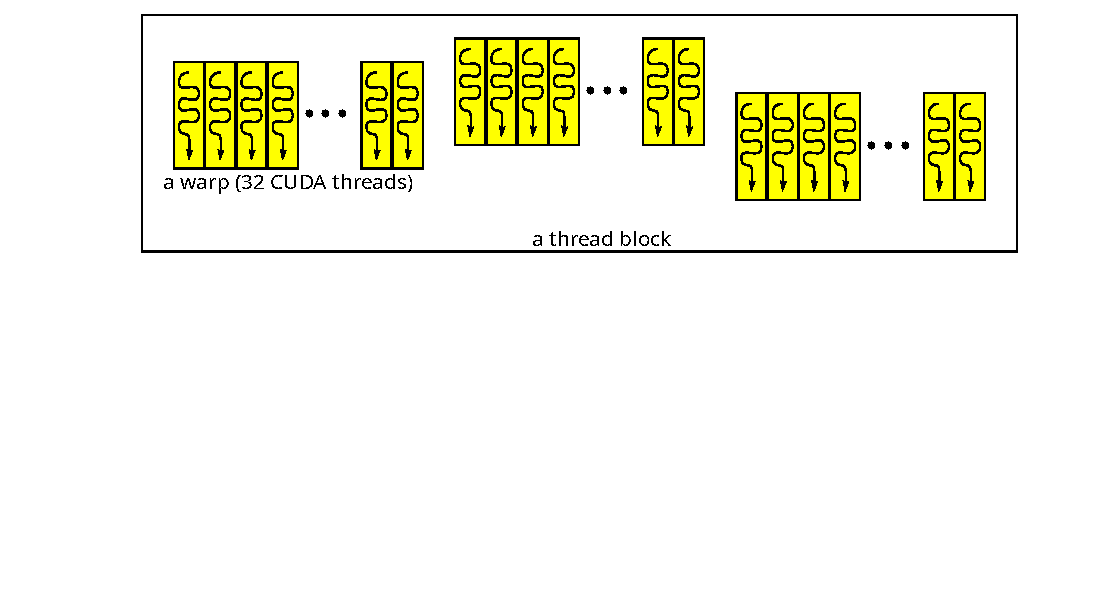
\includegraphics[width=0.7\textwidth]{out/pdf/svg/warp_block_sm_3.pdf}}%
    \only<4>{
\includegraphics[width=0.7\textwidth]{out/pdf/svg/warp_block_sm_4.pdf}}%
  \end{center}
\end{frame}

%%%%%%%%%%%%%%%%% 
\begin{frame}
  \frametitle{Warps}
  \begin{itemize}
  \item a warp is the unit of \ao{\it instruction execution}
  \item 32 threads in a single warp share an instruction pointer
    (a warp $\approx$ a CPU thread executing 32-way SIMD instructions)
  \item at every cycle, an SM selects a few (actually, $\leq 2$) warps and execute them
  \item $\Rightarrow$
    \begin{itemize}
    \item there is rarely a point in making {\em bs} $<$ 32
      or not a multiple of 32
      (ramainder threads consume resources but perform no useful work)
    \item you want to make 32 threads branch in the same way
      (avoid {\em warp divergence})
    \end{itemize}
  \end{itemize}

  \begin{center}
    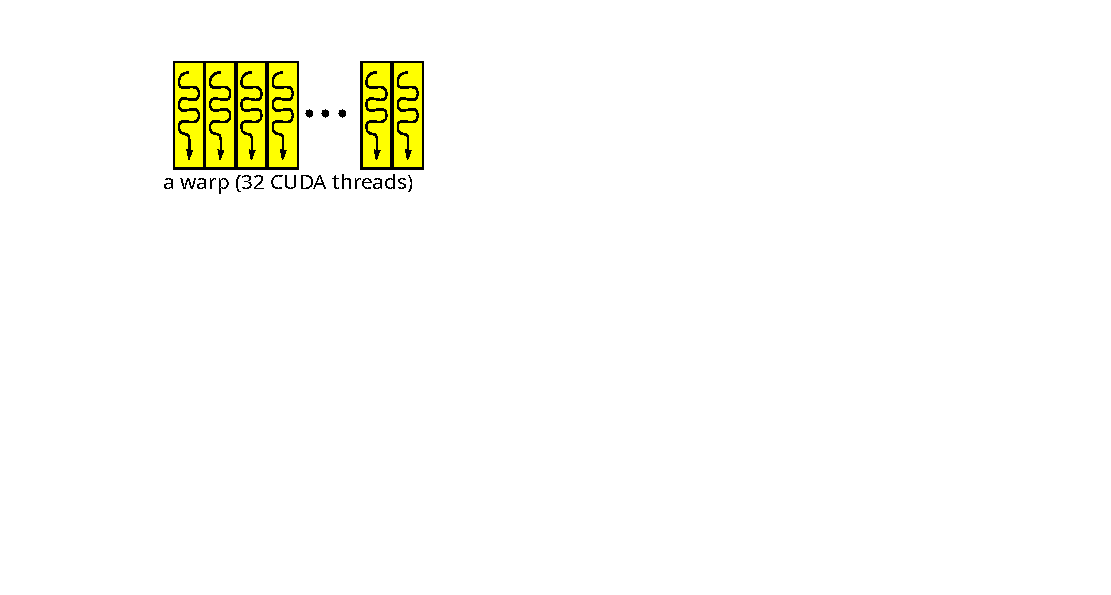
\includegraphics[width=0.7\textwidth]{out/pdf/svg/warp_block_sm_2.pdf}
  \end{center}
\end{frame}

%%%%%%%%%%%%%%%%% 
\begin{frame}
  \frametitle{Thread blocks}
  \begin{itemize}
  \item a thread block is \ao{\it the unit of dispatching to an SM}
  \item conceptually, a kernel launch {\tt f<<<{\it nb}, ...>>>(x, y, ...)}
    puts  {\it nb} blocks in a queue, which GPU dispatches to SMs,
    one block at a time
  \item once a block starts running, they stay on the SM \ao{\it until it finishes}
    and occupies \ao{\it registers} and \ao{\it shared memory} throughout
  \item $\Rightarrow$ the number of blocks {\it simultaneously} running on an SM
    is limited by registers and shared memory a thread block uses
  \end{itemize}
  \begin{center}
    
\includegraphics[width=0.7\textwidth]{out/pdf/svg/warp_block_sm_5.pdf}
  \end{center}
\end{frame}

%%%%%%%%%%%%%%%%% 
\begin{frame}[fragile]
  \frametitle{Registers and shared memory}
  \begin{itemize}
  \item registers
    \begin{itemize}
    \item hold \ao{\it local and temporary variables} of threads
    \item the size is determined by your program and the compiler
    \end{itemize}
  \item shared memory
    \begin{itemize}
    \item can be allocated when launching a kernel by
    \begin{lstlisting}
f<<<@{\it nb}@, @{\it bs}@, @\ao{$S_b$}@>>>(x, y, z, ...)
\end{lstlisting}
and is shared within a thread block
    \end{itemize}
  \end{itemize}
  \begin{center}
    
\includegraphics[width=0.7\textwidth]{out/pdf/svg/warp_block_sm_5.pdf}
  \end{center}
\end{frame}

%%%%%%%%%%%%%%%%% 
\begin{frame}
  \frametitle{Hardware limits}
  \begin{itemize}
  \item all numbers are per SM
  \item A100 (compute capability 8.0)
    \begin{tabular}{|l|r|}\hline
      registers & 65336 $\times$ 32 bits \\
      shared memory & 164 KB \\
      warps that can simultaneously run & 64 \\
      thread blocks that can simultaneously run & 32 \\\hline
    \end{tabular}
  \item V100 (compute capability 7.0)
    \begin{tabular}{|l|r|}\hline
      registers & 65336 $\times$ 32 bits \\
      shared memory & 96 KB \\
      warps that can simultaneously run & 64 \\
      thread blocks that can simultaneously run & 32 \\\hline
    \end{tabular}
  \end{itemize}
\end{frame}

%%%%%%%%%%%%%%%%% 
\begin{frame}
  \frametitle{Putting them together \\
    {\small blocks that will simultaneously run on an SM}}
  given (from the programmer or the compiler)
  \begin{itemize}
  \item $T_b$ : the number of threads per block,
  \item \mido{$S_b$} : \mido{shared memory} size per block, and
  \item $R_1$ : registers per thread,
  \end{itemize}
  calculate various resources {\it per block}
  \begin{itemize}
  \item \ao{\it warps} per block :
    $\ao{W_b} = \left\lceil T_b / 32 \right\rceil$
  \item \ore{\it registers} per block :
    $\ore{R_b} = 32R_1 \times W_b$
  \end{itemize}
  \begin{center}
    
\includegraphics[width=0.6\textwidth]{out/pdf/svg/warp_block_sm_5.pdf}
  \end{center}
\end{frame}


%%%%%%%%%%%%%%%%% 
\begin{frame}
  \frametitle{Putting them together}
  \begin{itemize}
  \item the number of blocks that simultaneously run on an SM ({\it nb})
    \begin{eqnarray*}
      \mbox{\it nb}
      & = & \mbox{min}(\left\lfloor 65536/R_b \right\rfloor, 
            \left\lfloor 164\mbox{K}/S_b \right\rfloor,
            \left\lfloor 64/W_b \right\rfloor,
            32) \\
      & = & \mbox{min}(\left\lfloor 2048/(R_1 W_b)\right\rfloor,
            \left\lfloor 164\mbox{K}/S_b\right\rfloor,
            \left\lfloor 64/W_b \right\rfloor, 32)
    \end{eqnarray*}
    
  \item the number of warps simultaneously run on an SM ({\it nw})
    \begin{eqnarray*}
      \mbox{\it nw}
      & = & W_b \cdot \mbox{\it nb} \\
      & = & W_b \cdot \mbox{min}(\left\lfloor 2048/(R W_b)\right\rfloor,
            \left\lfloor 164\mbox{K}/S_b\right\rfloor,
            \left\lfloor 64/W_b \right\rfloor, 32)
    \end{eqnarray*}
  \end{itemize}
  \begin{center}
    
\includegraphics[width=0.6\textwidth]{out/pdf/svg/warp_block_sm_5.pdf}
  \end{center}
\end{frame}

%%%%%%%%%%%%%%%%% 
\begin{frame}
  \frametitle{Takeaways (often good thread block sizes)}
  \[ W_b \cdot \mbox{min}(\left\lfloor 2048/(R_1 W_b)\right\rfloor,
    \left\lfloor 164\mbox{K}/S_b\right\rfloor,
    \left\lfloor 64/W_b \right\rfloor, 32) \]
  if we ignore factors that come from $R_1$ and $S_b$,
  a guideline is to run the maximum 64 warps simultaneously and it can be accomplished by
  \begin{itemize}
  \item putting at least two warps in a block (so $64/W_b \leq 32$) and 
  \item chooseing the number of warps per block that divides 64
  \item that is, $W_b = 2, 4, 8, 16, 32$
    (or $T_b = 64, 128, 256, 512, 1024$)
  \end{itemize}
\end{frame}

%%%%%%%%%%%%%%%%% 
\begin{frame}
  \frametitle{Remarks}
  \begin{itemize}
  \item 64 warps is merely {\it an} upper bound that
    \begin{itemize}
    \item may not be necessary to get the maximum performance (e.g., floating point
      performance, whose limit is 2-warp ($= 64$) FMAs per cycle) and
    \item may not be achievable due to other constraints (registers and shared memory)
    \end{itemize}
  \item the above takeaway is a rule of thumb to eliminate bad thread block sizes
  \end{itemize}
\end{frame}

%%%%%%%%%%%%%%%%% 
\begin{frame}
  \frametitle{Occupancy calculator}
  \begin{itemize}
  \item NVIDIA used to provide a simple
    \href{https://docs.nvidia.com/cuda/cuda-occupancy-calculator/index.html}{Excel} to give you how many warps
    can run simultaneously given block size ($T_b$), shared memory per block ($S_b$), and
    registers per thread ($R_1$)
    
  \item a small web page doing the same at
    \url{https://xmartlabs.github.io/cuda-calculator/}
    
  \end{itemize}
\end{frame}

\end{document}



%%%%%%%%%%%%%%%%% 
\begin{frame}[fragile]
  \frametitle{Shared memory}
  \begin{itemize}
  \item recall that a thread block may use {\it shared memory}
    and the programmer can specify its size per block ($S_b$ below)
    \begin{lstlisting}
f<<<@{\it nb}@, @{\it bs}@, @$S_b$@>>>(x, y, z, ...)
    \end{lstlisting}
  \item each SM has a fixed amount of shared memory (A100 has 164KB), 
    which limits the number of blocks that can run simultaneously on an SM
  \end{itemize}
\end{frame}

%%%%%%%%%%%%%%%%% 
\begin{frame}
  \frametitle{Registers/shared memory and parallelism}
  \begin{itemize}
  \item Q. how many thread blocks execute simultaneously?
  \item A. it is subject to resource constraints.  say $N$ is the number of simultaneously executing thread blocks on an SM
    \begin{itemize}
    \item registers
      \[ R \times \mbox{\it bs} \times N \leq \mbox{registers per SM} \]
    \item shared memory
      \[ S \times N \leq \mbox{shared memory per SM} \]
    \end{itemize}
  \item GPU determines it appropriately based on register
    and shared memory usage
  \end{itemize}

  \begin{center}
    
\includegraphics[width=0.5\textwidth]{out/pdf/svg/warp_block_sm_4.pdf}
  \end{center}
\end{frame}




%%%%%%%%%%%%%%%%% 
\begin{frame}
  \frametitle{}
  \begin{itemize}
  \item all threads are first grouped into 32-thread groups, called warps
    \begin{itemize}
    \item threads of ID 0..31 makes a warp, 32..63 makes another, etc.
    \end{itemize}
  \item 32 threads in a single warp share a single instruction pointer
    and therefore always execute the same instruction together in a cycle

  \item all warps in the same thread block are dispatched together to
    an SM and, once started, reside in that SM until all warps in the
    block are finished
    
  \end{itemize}
\end{frame}

%%%%%%%%%%%%%%%%% 
\begin{frame}
  \frametitle{How to choose a block size (threads per block)}
  \begin{itemize}
  \item when you have a fixed number of threads,
    how to divide them into blocks?
  \item a general goal is to run a large enough number of threads
    {\em simultaneously} on each SM
  \item some important concepts
    \begin{itemize}
    \item warp (32 threads that share an instruction pointer register)
    \item each SM has only so many registers/shared memory
    \end{itemize}
  \end{itemize}
\end{frame}

%%%%%%%%%%%%%%%%% 
\begin{frame}
  \frametitle{An abstract model of how GPU determines the number of
  thread blocks running at the same time}
  \begin{itemize}
  \item input
    \begin{itemize}
    \item threads per block ({\it bs})
    \item (32 bit) registers per thread ($R$)
      \begin{itemize}
      \item a 64 bit number is counted as two
      \end{itemize}
    \item shared memory per thread block ($S$)
    \end{itemize}
  \item output
    \begin{itemize}
    \item $n = $ how many thread blocks a single SM can execute simultaneously
    \end{itemize}
  \item $n$ is the minimum of the three
    \begin{itemize}
    \item $\left\lceil 65536 / (R \times \mbox{\it bs}) \right\rceil$
    \item $\left\lceil \mbox{164KB} / S \right\rceil$
    \item 16
    \item $48 / \left\lceil \mbox{\it bs} / 32 \right\rceil$
    \end{itemize}
    
  \end{itemize}
\end{frame}

%%%%%%%%%%%%%%%%% 
\begin{frame}
  \frametitle{How to choose a block size (threads per block)}
  \begin{itemize}
  \item absolute constraints on the thread block size (\ao{\it bs})
    \begin{itemize}
    \item {\it a constant limit} : $\mbox{\it bs} \leq 1024$ (on P100 and V100)
    \item {\it registers}
    \end{itemize}
  \item performance considerations: parallelism within an SM
    \begin{itemize}
    \item \ao{\it warp}
    \item \ao{\it registers}
    \item \ao{\it shared memory}
    \end{itemize}
  \item performance considerations: parallelism across SMs
  \end{itemize}
\end{frame}

%%%%%%%%%%%%%%%%% 
\begin{frame}
  \frametitle{Registers}
  \begin{itemize}
  \item a thread consumes a number of (say $R$) registers
    to hold \ao{\it local and temporary variables}
  \item a thread block therefore consumes accordingly many registers,
    \ao{\it throughout its lifetime (from the beginning to the end)}
  \item each SM has a fixed amount of registers
    (32 bit $\times$ 65536, both on P100 and V100)
  \item as each SM obviously needs to accommodate at least one thread block,
    you must have
    \[ R \times \mbox{\it bs} \leq 65536 \]
  \end{itemize}
\end{frame}

%%%%%%%%%%%%%%%%% 
\begin{frame}
  \frametitle{Registers/shared memory and parallelism}
  \begin{itemize}
  \item Q. how many thread blocks execute simultaneously?
  \item A. it is subject to resource constraints.  say $N$ is the number of simultaneously executing thread blocks on an SM
    \begin{itemize}
    \item registers
      \[ R \times \mbox{\it bs} \times N \leq \mbox{registers per SM} \]
    \item shared memory
      \[ S \times N \leq \mbox{shared memory per SM} \]
    \end{itemize}
  \item GPU determines it appropriately based on register
    and shared memory usage
  \end{itemize}

  \begin{center}
    
\includegraphics[width=0.5\textwidth]{out/pdf/svg/warp_block_sm_4.pdf}
  \end{center}
\end{frame}

\iffalse
%%%%%%%%%%%%%%%%% 
\begin{frame}
  \frametitle{Restrictions affecting the correctness}
  \begin{itemize}
  \item \aka{\it you cannot make a single thread block arbitrarily large}
    \begin{itemize}
    \item for P100, 

\begin{tabular}{rcl}
  \aka{{\it bs}} & $\leq$ & \aka{1024} \\
  \aka{{\it bs} $\times$ {\it R}} & $\leq$ & \aka{65536} \\
\end{tabular}
\item [] $R = $ the number of {\it registers} used per thread
\end{itemize}
\item GPU has a faster memory, \ao{\it shared memory},
  which is \aka{\it only shared within a single thread block}
  \begin{itemize}
  \item it's more like a scratch pad memory (it's a misnomer IMO)
  \end{itemize}
\end{itemize}

\begin{center}
  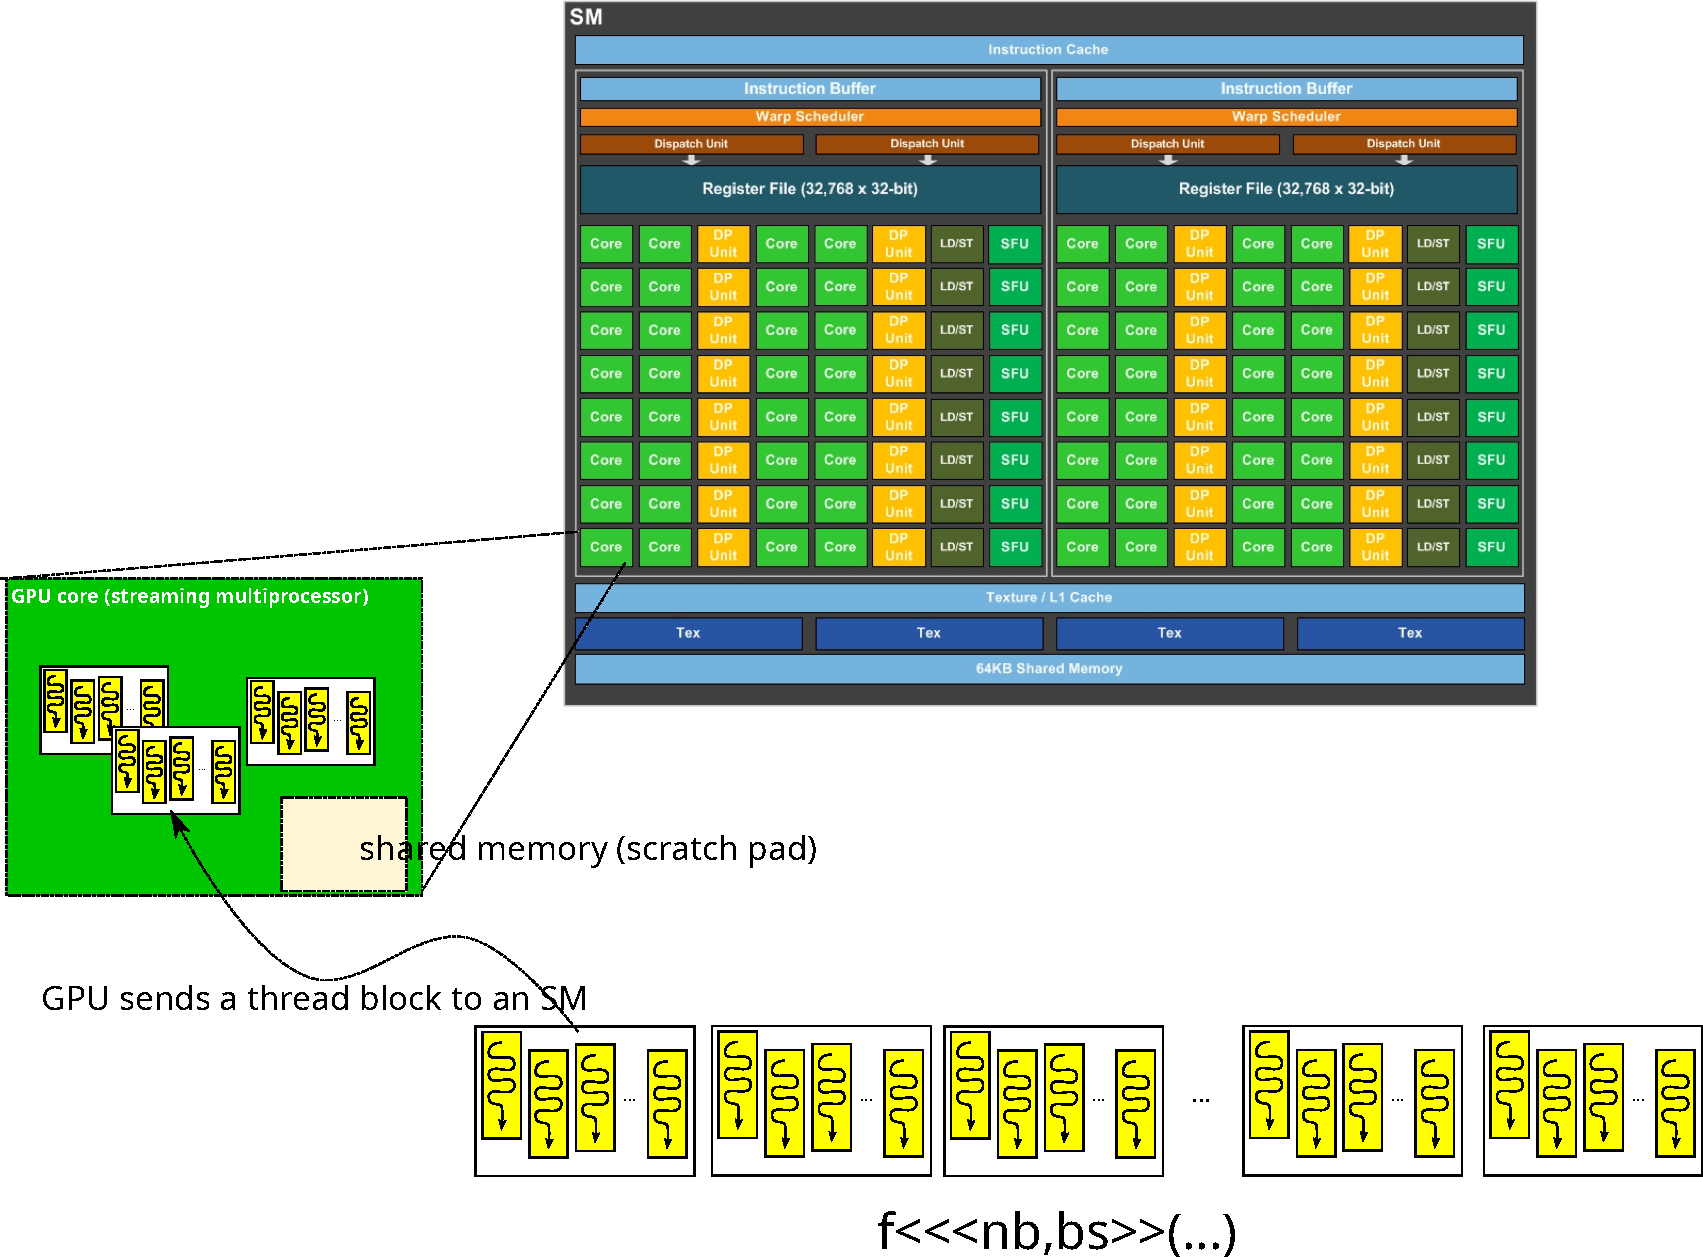
\includegraphics[width=0.45\textwidth]{out/pdf/svg/sm_and_blocks_2.pdf}
\end{center}

\end{frame}

%%%%%%%%%%%%%%%%% 
\begin{frame}
  \frametitle{About registers}
  \begin{itemize}
  \item each SM has a number of (65536 on P100) registers
  \item for an SM to accommodate at least one thread block,
    it must hold 
    \[ \aka{\mbox{\it bs} \times R \leq 65536}, \]
    where $R$ is the number of registers used per thread
  \item how you can know $R$? $\rightarrow$
    pass {\tt -Xptxas -v} to {\tt nvcc} and see the compiler message
  \item can you control it? $\rightarrow$ pass
    {\tt --maxrregcount} $R$ to {\tt nvcc}
  \end{itemize}
\end{frame}

%%%%%%%%%%%%%%%%% 
\begin{frame}
  \frametitle{Factors affecting performance}
  \begin{itemize}
  \item to utilize multiple (many) SMs,
    you want to create accordingly many thread blocks
  \item to efficiently use a single SM,
    you want to have enough threads in each SM
  \item how to choose them affects performance (later weeks)
  \end{itemize}

  \begin{center}
    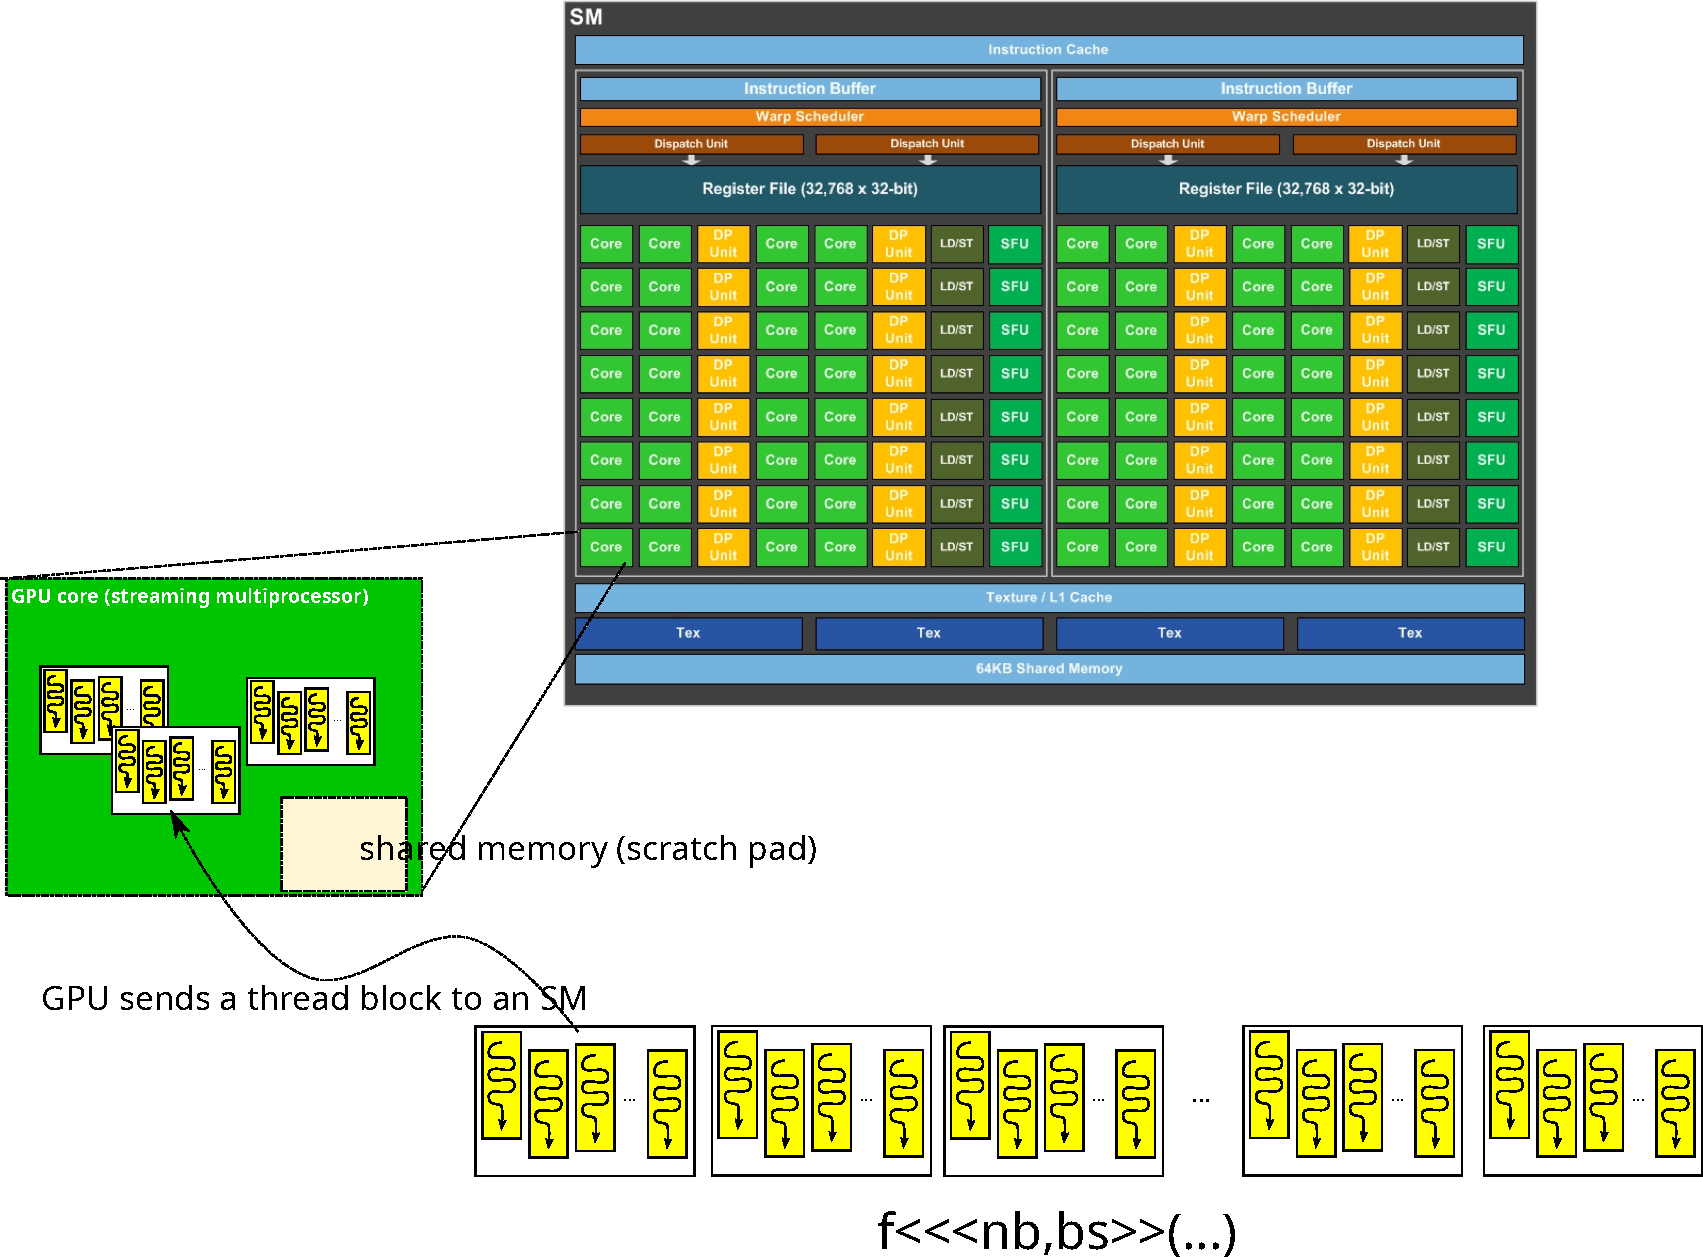
\includegraphics[width=0.6\textwidth]{out/pdf/svg/sm_and_blocks_2.pdf}
  \end{center}
\end{frame}

%%%%%%%%%%%%%%%%% 
\begin{frame}
  \frametitle{Tips to choose a right thread block size, for now}
  \begin{itemize}
  \item make it a multiple of 32 (warp size) and $\leq$ 1024
    \begin{itemize}
    \item 32, 64, 96, $\cdots$, 1024
    \end{itemize}
  \item complex kernels may fail with a large block size.
    reduce it when it happens
    \begin{itemize}
    \item always check a launch error at runtime!
    \item see compiler message {\tt -Xptxas -v} and control it when necessary
      {\tt --maxrregcount} 
    \end{itemize}
    
  \item small threads need more of them to fill an SM
  \end{itemize}
\end{frame}
\fi
    
\end{document}

